
\def\year{2019}\relax
%File: formatting-instruction.tex
\documentclass[letterpaper]{article} %DO NOT CHANGE THIS
\usepackage{aaai19}  %Required
\usepackage{times}  %Required
\usepackage{helvet}  %Required
\usepackage{courier}  %Required
\usepackage{url}  %Required
\usepackage{graphicx}  %Required
\frenchspacing  %Required
\setlength{\pdfpagewidth}{6.5in}  %Required
\setlength{\pdfpageheight}{11in}  %Required
\pdfinfo{
/Title (Updates in Human-AI Teams: The Performance/Compatibility Tradeoff)
/Author (Gagan Bansal, Besmira Nushi, Ece Kamar, Daniel S. Weld, Walter S. Lasecki, Eric Horvitz)}
\setcounter{secnumdepth}{1}  

%%%%%%%% custom commands %%%%%%%%
\usepackage{subcaption}
\usepackage{booktabs} % For formal tables
\usepackage{float}
\usepackage{todonotes}
\usepackage{enumitem}
\usepackage{bbm}
\usepackage{url}
\renewcommand{\UrlFont}{\ttfamily\small}
\usepackage{soul}
% \usepackage{subfigure}
\usepackage{relsize}

\renewcommand*{\UrlFont}{\ttfamily\smaller\relax}



% \usepackage{amsmath,amssymb}

%%%%%%%%%%%%  change tracking below here
\usepackage[english]{babel}
%\usepackage[dvipsnames,svgnames,x11names]{xcolor}
\usepackage[markup=underlined]{changes}
%% Use "final" option to remove all tracking markups
% \usepackage[final]{changes}
%\definechangesauthor[color=BrickRed]{EH}
%\definechangesauthor[color=NavyBlue]{DW}

%%% Alternative definition to have the remarks
%%% in the margins instead of footnotes
\usepackage{todonotes}
%\setlength{\marginparwidth}{3cm}
\makeatletter
\setremarkmarkup{\todo[color=Changes@Color#1!20,size=\scriptsize]{#1: #2}}
\makeatother

%% Rather hacky definition of a plain remark/note
%% by riding on \added
\newcommand{\note}[2][]{\added[#1,remark={#2}]{}}
%%%%%%%%% end change tracking defns


\newcommand{\NOTE}[1]{\marginpar{\em {#1}}}
\newcommand{\bug}
    {\mbox{\rule{2mm}{2mm}}}
\newcommand{\Bug}[1]
    {\bug \footnote{BUG: {#1}}}
\newcommand{\QED}{\mbox{$\Box$}}
\newcommand{\ddt}{\mbox{$\frac{d}{dt}\,$}}  %* no strut

\newcommand{\etal}{\mbox{\it et al.}}
\newcommand{\etc}{\mbox{\it etc.}}
\newcommand{\eg}{\mbox{\it e.g.}}
\newcommand{\ie}{\mbox{\it i.e.}}
\newcommand{\cf}{\mbox{\it cf.}}
\newcommand{\Eg}{\mbox{\it E.g.}}
\newcommand{\Ie}{\mbox{\it I.e.}}
\newcommand{\?}{\mbox{?}}




\newcommand{\DEFN}{\mbox{$\stackrel{\mbox{\tiny def}}{=}$}}

\newcommand{\TT}[1]{\mbox{\tt #1}}
%\newcommand{\bi}{\begin{itemize}}
%\newcommand{\ei}{\end{itemize}}
\newcommand{\bi}{\begin{list}{$\bullet$}{
    \setlength{\leftmargin}{1.5 em}
    \setlength{\itemsep}{0 pt}
    \setlength{\topsep}{3 pt}
    \setlength{\parsep}{3 pt}
    \setlength{\partopsep}{0 pt}
    \setlength{\labelwidth}{1 em}
    \setlength{\labelsep}{0.5 em}
    \setlength{\parskip}{0cm}  }}
\newcommand{\ei}{\end{list}}

\newcommand{\BE}{\begin{enumerate}}
\newcommand{\EE}{\end{enumerate}}

%\newtheorem{defnctr}{Definition}
%\newtheorem{theorem}{Theorem}
%\newtheorem{lemma}[theorem]{Lemma}
%\newtheorem{corollary}[theorem]{Corollary}        
%\newtheorem{conjecture}[theorem]{Conjecture}
%\newtheorem{propos}[theorem]{Proposition}
%\newcommand{\proof}
%	{\vspace{-8pt}
%	 {\bf Proof:}}



\newcommand{\tuple}[1]
        {\mbox{$\langle{#1}\rangle$}}
\newcommand{\set}[1]
        {\mbox{$\{{#1}\}$}}
\newcommand{\size}[1]{\mbox{$\mid\!#1\!\mid$}}



\newcommand{\PROOF}[1]{\mbox{\noindent \proofbegin {#1} \proofend}}
\newcommand{\proofbegin}{\mbox{\bf Proof: \ }}
\newcommand{\proofend}{\Math{\Box}}
%\newcommand{\st}{\mbox{ such that }}
\newcommand{\wht}{\mbox{ we have that }}
\newcommand{\entails}{\mbox{$\models$}}
\newcommand{\yields}{\mbox{$\models$}}
\newcommand{\dgets}{\mbox{$\leftarrow$}}





\newcommand{\initab}{                           % set up tab stops
\begin{tabbing}
XXX \= XXXX \= \kill
}
\newcommand{\begpub}{
\begin{quotation}
\noindent
}
\newcommand{\nextpub}{

\vspace{2mm}
\noindent
}
\newcommand{\finpub}{
\end{quotation}
}



\hyphenation{non-de-ter-mi-nis-tic-al-ly non-de-ter-mi-nis-tic
exis-ten-tial-ly quan-tified se-lec-tion exis-ting in-stan-tiated
uni-vers-al-ly es-tab-lish in-con-sis-tent class-ifier}


% \newcommand{\ncd}{\mbox{$\neq$}}
% \newcommand{\cd}{\mbox{$=$}}
% \newcommand{\fabian}{\mbox{\sc fabian}}
% \newcommand{\occam}{\mbox{\sc occam}}
% \newcommand{\sadl}{\mbox{\sc sadl}}
% \newcommand{\socrates}{\mbox{\sc socrates}}
% \newcommand{\uwl}{\mbox{\sc uwl}}
% \newcommand{\spa}{\mbox{\sc spa}}
% \newcommand{\scr}{\mbox{\sc scr}}
% \newcommand{\strips}{\mbox{\sc strips}}
% \newcommand{\snlp}{\mbox{\sc snlp}}
% \newcommand{\cbur}{\mbox{\sc C-buridan}}
% \newcommand{\buridan}{\mbox{\sc buridan}}
% \newcommand{\xii}{\mbox{\sc xii}}
% \newcommand{\zeno}{\mbox{\sc zeno}}
% \newcommand{\adl}{\mbox{\sc adl}}
% \newcommand{\kr}{\mbox{\tt /kr94}}
% \newcommand{\ucpop}{\mbox{\sc ucpop}}
% 
% \newcommand{\cause}{{\tt cause}}
% \newcommand{\observe}{{\tt observe}}
% \newcommand{\satisfy}{{\tt satisfy}}
% \newcommand{\handsoff}{{\tt hands-off}}
% \newcommand{\findout}{{\tt find-out}}
% 
% \newcommand{\CAUS}{\mbox{C}}
% \newcommand{\OBS}{\mbox{O}}
% \newcommand{\PAT}{\mbox{\sf E}}
% \newcommand{\fact}{\mbox{$\varphi$}}
% \newcommand{\LIT}{\mbox{\sf p}}
% \newcommand{\lit}{\mbox{\LIT}}
% \newcommand{\litp}{\mbox{\LIT$^\prime$}}
% \newcommand{\rel}{\mbox{REL}}
% \newcommand{\change}[3]{\mbox{$\Delta(#1,{\tt #2}\rightarrow {\tt #3})$}}   
% 
% \newcommand{\true}{{\tt T}}
% \newcommand{\false}{{\tt F}}
% \newcommand{\unknown}{{\tt U}}
% 
%

% Notation macros
\newcommand{\name}{AI-advised human decision making}
\newcommand{\plat}{{\sc Caja}}
\newcommand{\hone}{\mbox{$h_1$}}
\newcommand{\htwo}{\mbox{$h_2$}}
\newcommand{\dtrainone}{\mbox{$D_1$}}
\newcommand{\dtraintwo}{\mbox{$D_2$}}
\newcommand{\dtrain}{\mbox{$D_{\text{train}}$}}  % use of \mbox means macro will work both inside or outside of math mode
\newcommand{\dtest}{\mbox{$D_{\text{test}}$}}
\newcommand{\compatscore}{\mathcal{C}}
\newcommand{\loss}{L}
\newcommand{\lossbc}{\loss_c}
\newcommand{\lambdabc}{\lambda_c}
\newcommand{\dissonance}{\mathcal{D}}
\newcommand{\err}{\textit{err}}


\usepackage{amsmath}
\usepackage{amsthm}
\usepackage{amssymb}
\newtheorem*{definition}{Definition}
\newtheorem*{example}{Example}

\title{Updates in Human-AI Teams:\\ Understanding and Addressing the Performance/Compatibility Tradeoff}
% \author{Submission: 6666}
\author{
Gagan Bansal,\textsuperscript{\rm 1}
Besmira Nushi,\textsuperscript{\rm 2}
Ece Kamar,\textsuperscript{\rm 2}
Daniel S. Weld,\textsuperscript{\rm 1}
Walter S. Lasecki,\textsuperscript{\rm 3}
Eric Horvitz\textsuperscript{\rm 4}\\
\textsuperscript{\rm 1}University of Washington,
\textsuperscript{\rm 2}Microsoft Research,
\textsuperscript{\rm 3}University of Michigan
}

%\author{
%John Wang,\textsuperscript{\rm 1}
%Gerald Jones,\textsuperscript{\rm 2}
%Xiaojuan Yang,\textsuperscript{\rm 3}
%Xiao Liu,\textsuperscript{\rm 4}
%Katherine Ross\textsuperscript{\rm 1}\\
%\textsuperscript{\rm 1}The XYZ University,
%\textsuperscript{\rm 2}The Company\\
%\textsuperscript{\rm 3}University of Artificial Intelligence,
%\textsuperscript{\rm 4}Country University of Finance and Economics\\
%author1@lab.org, author2@gmail.com, author3@university.edu. 
%author4@mail.company.cn, author5@nonprofit.org
%}

\begin{document}
\maketitle

\begin{abstract}

AI systems are being deployed to support human decision making in high-stakes domains such as healthcare and criminal justice. In many cases, the human and AI form a team, in which the human makes decisions after reviewing the AI's inferences. A successful partnership requires that the human develops insights into the performance of the AI system, including its failures. We study the influence of {\em updates} to an AI system in this setting. While updates can increase the AI's predictive performance, they may also lead to behavioral changes that are at odds with the user's prior experiences and confidence in the AI's inferences. We show that updates that increase AI performance may actually hurt {\em team} performance. 
We introduce the notion of the {\em compatibility} of an AI update with prior user experience and present methods for studying the role of compatibility in human-AI teams. 
Empirical results on three high-stakes classification tasks show that current machine learning algorithms do not produce compatible updates. We propose a re-training objective to improve the compatibility of an update by penalizing new errors. The objective offers full leverage of the performance/compatibility tradeoff across different datasets, enabling more compatible yet accurate updates.

%The proposed objective significantly improves compatibility by trading it off with accuracy across different datasets.

%When people rely on AI systems to make decisions, they need to understand the accuracy of the AI's inferences.
%Previous studies have shown that as people interact with AI, they develop insights about its successes and failures. 
%We consider the challenge of human-AI collaboration when, over time, the AI changes.
%For example, developers regularly update systems: Siri and Cortana, today, aren't the same agents they were last month.
%While updates can increase the AI's predictive performance, they can lead to changes in behavior that  are at odds with the user's %prior experiences and confidence in inferences.
%Updates that increase performance may actually hurt {\em team} performance. 

% AI can augment humans, and such human-AI teams may perform better than either teammate alone. However, for humans to effectively collaborate with an (imperfect) AI, they must understand when to trust it. Indeed, cognitive science research shows that, as humans interact with the AI, they develop a better understanding of it. 
% However, developers regularly update systems: Siri and Cortana, today, aren't the same agents they were last month.
% While updates usually increase the AI's absolute performance, they can disrupt the human's understanding and actually hurt {\em team} performance. 

% We introduce the notion of compatibility of an update to an AI and develop a platform to study the impact of compatibility on team performance. Studies show that a more accurate, but incompatible AI can perform worse than a less accurate, but more compatible AI. Then, on three high-stakes classification tasks, we show that current ML pipelines do not produce compatible updates. To address this, we propose a practical (re)training objective to improve the compatibility of an update. Our method penalizes hypotheses that introduce new errors. This method reveals a trade-off between the performance of AI and its compatibility.
% \vspace*{-0.6}
\end{abstract}

%\keywords{Human-AI teams, AI safety and reliability, mental models, explainable AI} 

\maketitle

%Candidate Titles
%\begin{itemize}
%\item Model Updates and AI-Human Teams: Introducing Considerations of Prior Experience and Expectations
%\item Updates in AI-Human Teams: Navigating the Performance/ Compatibility Tradeoff
%\item Updating Human-Facing AI: The Accuracy/Compatibility Tradeoff
%\item Updating Human-Facing AI: The Performance/Compatibility Tradeoff
%\item A Case for Backward Compatibility in Machine Learning 
%\item Managing the Tradeoff Between Compatibility and Accuracy for Human-AI Teams
%\item Human-AI Teams and Accuracy-Compatibility Tradeoff
%\item The Ever-changing Face of AI 
% \Bug{WSL: something like this... or maybe too "cute"?\\G: I like it. Dan at some point suggested something similar by using the word "Schizophrenia"}
%\item Updates in AI-Human Teams: The Accuracy/Compatibility Tradeoff}
%\item Model Updates and AI-Human Teams: Introducing Considerations of Backward Compatability
%\end{itemize}


\section{Introduction}

A promising opportunity in AI is developing systems that can partner with people to accomplish tasks in ways that exceed the capabilities of either individually~\cite{wang2016deep,kamar2016directions,gaur2016effects}.
We see many motivating examples: a doctor using a medical expert system~\cite{wang2016deep}, a judge advised by a recidivism predictor, or a driver supervising a semi-autonomous vehicle. Indeed, economists expect human-AI teams to handle many such tasks~\cite{forrester-17}. Despite rising interest, there is much to learn about creating effective human-AI teams and what capabilities AI systems should employ to be competent partners. 

\begin{figure}[t]
    \begin{center}
    % \missingfigure[figwidth=6cm]{}
    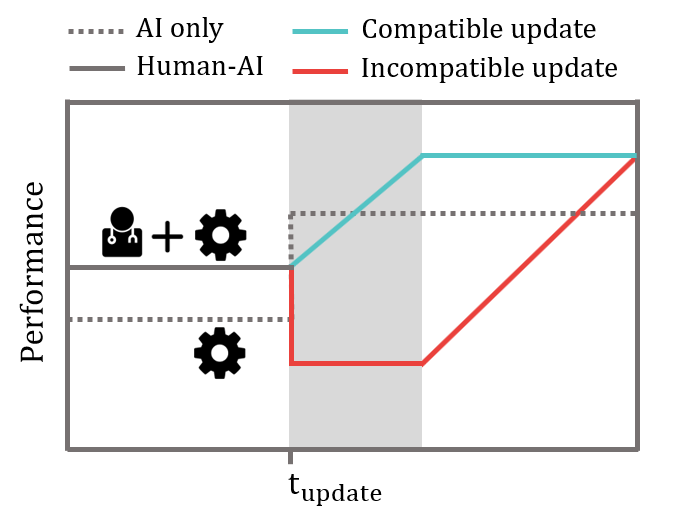
\includegraphics[width=\linewidth]{Picture1v2.png}
    \end{center}
    %\vspace{-1pc}
    \caption{Schematized view of human-AI teams in the presence of AI updates. Human-AI teams perform better than either alone, but when the AI is {\em updated} its behavior may violate human expectations. Even if updates increase the AI's {\em individual} performance, they may reduce {\em team} performance by making mistakes in regions where humans have learned to trust the AI.}
    %\vspace*{-0.8pc}
    %\Bug{The blue needs to fix: it shouldn't be flat} }
    \label{fig:landing}
\end{figure}

We study human-AI teams in decision-making settings where a user takes action recommendations from an AI partner for solving a complex task. The user considers the recommendation and, based on previous experience with the system, decides to accept the suggested action or take a different action. We call this type of interaction {\em AI-advised human decision making}. While there exist other important forms of human-AI collaboration (including human-advised AI decision making and more general collaborative decision making involving a mix of initiatives and emergent team behaviors), we focus on a specific interplay where the goal is to create AI systems that recommend actions to assist humans with decisions in high-stakes domains~\cite{angwin2016machine,bayati2014data}. The motivation for AI-advised human decision making comes from the fact that humans and machines have complementary strengths and abilities. While both human experts and machine-learned models are not perfect on a task like medical diagnosis or classifying objects in images, researchers have shown that their ideal combination could significantly improve performance~\cite{wang2016deep,kamar2012combining}. 
AI systems offer added benefits by speeding up decision making when humans can identify tasks where the AI can be trusted and no more human effort is needed~\cite{lasecki2012scribe,lasecki2012real}. 
%Moreover, AI systems offer additional benefits by speeding up decision making in cases where humans can easily identify tasks with which the AI can be trusted and no further human effort or analysis is needed~\cite{lasecki2012scribe,lasecki2012real}. 
% \Bug{\sout{Add motivation. EK: I took a pass. G: looks great to me, striking it out}}

It might be expected that improvements in the performance of AI systems lead to stronger team performance, but, as with human groups, individual ability is only one of many factors that affect team effectiveness~\cite{dechurch-jap10,grosz1996collaborative}. Even in a simple collaboration scenario, in which an AI system assists a human decision maker with predictions, the success of the team hinges on the human correctly deciding when to follow the recommendation of the AI system and when to override. Unless the particular domain and the interaction allows the human to validate the correctness of the machine recommendation efficiently and effectively, extracting benefits from collaboration with the AI system depends on the human developing insights (i.e., a mental model) of when to trust the AI system with its recommendations. If the human mistakenly trusts the AI system in regions where it is likely to err, catastrophic failures may occur. 
Human-AI teams become especially susceptible to such failures because of discrepancies introduced by system updates that do not account for human expectations. The following example and Figure~\ref{fig:landing} illustrate this situation.

%It might be expected that improvements in the performance of AI systems lead to stronger team performance, but, as with human groups, individual ability is only one of many factors that affect team effectiveness~\cite{dechurch-jap10,grosz1996collaborative}. Even in a simple collaboration scenario, in which an AI system assists a human decision maker with predictions, the success of the team hinges on the human developing insights about when to trust the decision of the AI system and when to override. In particular, mistakenly trusting the AI system in regions where it is likely to err can lead to costly failures. Human-AI teams are especially susceptible to such discrepancies following system updates that do not account for human expectations. The following example and Figure~\ref{fig:landing} illustrate this situation.

\begin{example}[\sc{Patient readmission}]
A doctor uses an AI system that is 95\% accurate at predicting whether a patient will be readmitted following their discharge to make decisions about enlisting the patient in a supportive post-discharge program. The special program is costly but promises to reduce the likelihood of readmission. After a year of interacting with the AI, the doctor develops a clear mental model that suggests she can trust the AI-advised actions on elderly patients. In the meantime, the AI's developer trains and deploys a new 98\% accurate classifier, which errs on elderly patients. 
While the AI has improved by 3\%, the doctor is unaware of the new errors, and as a result of this outdated mental model, takes the wrong actions for some elderly patients.
% \vspace*{-0.2pc}
\end{example}
% \Bug{Jim- clarify the example on patient readmission. It wasn't clear that doctor can reject a recommendation and that there is a cost to doing the task themselves}

This example is motivated by real-world AI applications for reducing patient readmissions and other costly outcomes in healthcare~\cite{bayati2014data,wiens2016patient,caruana2015intelligible}, and motivates the need for reducing the cost of disruption caused by updates that violate  %incompatible with 
users' mental models. The problem with updates extends to numerous AI-advised human decision-making settings; similar challenges have been observed during over-the-air updates in the Tesla autopilot~\cite{tesla:2018}, and  analogous issues arise in a variety of other settings when AI services 
being consumed by third-party applications, are updated.

Despite these problems, developers have almost exclusively optimized for AI performance.  Retraining techniques largely ignore important details about human-AI teaming, and the mental model that humans develop from interacting with the system. %  faithful to previous successful human-AI interactions. 
The goal of this work is to make the human factor a first-class consideration of AI updates. We make the following contributions: 

%For example, Microsoft Cognitive Services\footnote{\url{https://azure.microsoft.com/en-us/services/cognitive-services/}} may deploy its most accurate image classifier to date as a Web service. While the current version of the classifier is in production, they may gather more training data, train an even more accurate classifier, and then ``push'' the new version. Developers assume that if the AI improves the team performance will improve. However, this assumption may not always hold: What if the updated AI errs on the inputs on which the human trusted the previous version \Bug{we need a more clear setup here for readers -- i.e., some system that uses human-Ai teams is using this API, the API updates without knowing that, and the team gets worse}? What if the update introduces new errors in a classifier built for medical diagnosis?

% We find that more accurate AI does not always lead to better team performance in the short term, and we present methods for updating a machine-learning model while maintaining consistency with prior behavior.
%\Bug{Tesla citations: (1) https://www.theverge.com/2018/6/2/17413732/tesla-over-the-air-software-updates-brakes (2) https://teslamotorsclub.com/tmc/threads/software-update-version-2018-2.107164/  The second link is a discussion between Tesla owners wondering how Tesla got updated}


 %Many other factors likely impact the capability of a human-AI team, including the efficiency of the communication medium between human and AI %(\eg, brain interface), and the degree to which the human and the AI understand each other \cite{gunning2017explainable}. In recent years, the explainable AI (XAI) researcher community has investigated this last factor, developing algorithms for communicating to humans the rationale behind an AI's decisions. If humans understand the AI, they can collaborate more effectively; for example, they can reason about when to (and when not to) trust the AI's decision.


%Indeed, cognitive science research shows that when people collaborate with an  automated system, they create a mental model of it~\cite{rouse1986looking,rouse1992role,schumacher1992mental}. People use these models to describe, explain, and predict system behaviour. In the case of a human-AI team, people create models of the AI's competence: when is it correct and thus trustworthy.  For example, people reason about when it is appropriate to trust their spam filter and their self-driving car. In reality, such a competence model is imperfect and limited by the number of rounds of interaction, the system complexity, and human's cognitive limitations. Nevertheless, it is crucial: Better competence model would lead to higher team performance as the human partner would know when to trust the decisions of an AI system. Conversely, a wrong mental model can cause a human to trust the AI when she should not.

\begin{itemize}
\item We define the notion of compatibility of an AI update with the user's mental model created from past experience.
We then propose a practical adjustment to current ML (re)training algorithms --- an additional differentiable term to the logarithmic loss --- that improves compatibility during updates, 
and allows developers to explore the performance/compatibility tradeoff.
% \Bug{Need to distinguish between local and global -- list both here, but say focus is on global} %Based on this definition, 
%This term allows developers to explore the performance/compatibility trade-off according to the domain requirements.

\item We introduce an open-source experimental platform\footnote{Available at \url{https://github.com/gagb/caja}} for 
studying how people model the error boundary of an AI teammate in the presence of updates for a an AI-advised decision-making task. %Since it is challenging to study human mental models, 
The platform exposes important design factors (\eg, task complexity, reward, update type) to the experimenter. 
%Results confirm that in a team context, a less accurate but more predictable AI system may be more useful than one that is more accurate yet less predictable.
%\Bug{E: Check if there are any controlled studies of humans developing mental models. If not, this is a good contribution to list. If prior studies exist, we need to cite. Overall, we need to go over the literature Mary shared at the beginning of  the internship}

\item Using the platform, we perform user studies showing that, humans develop mental models of AI systems across different conditions, and that more accurate mental models improve team performance. More importantly, we show that updating an AI to increase accuracy, at the expense of compatibility, may {\em degrade} team performance. 
 Moreover, experiments on three high-stakes classification tasks (recidivism prediction, in-hospital mortality prediction, and credit-risk assessment) demonstrate that: (i) current ML models are not inherently compatible, but (ii) flexible performance/compatibility tradeoffs can be effectively achieved via a reformulated training objective.

%\item Leveraging the platform, we perform \Bug{need to highlight result that improved AI can lead to worse team performance and note statistical significance}
%user studies showing that, in a team context, predictable error boundaries and compatible updates can lead to improved team performance while updating to a more accurate but incompatible system may hurt the team performance.  Moreover, experiments on three high-stakes classification tasks (recidivism prediction, in-hospital mortality prediction, and credit-risk assessment) demonstrate that: (i) current ML models are not inherently compatible, but (ii) flexible performance/compatibility tradeoffs can be effectively achieved via a reformulated training objective.

%\item We make all code and datasets available open source, including the experimental platform for user studies.
%\footnote{Available at \url{https://github.com/gagb/caja}}
\end{itemize}


%\section{Problem Setting: Human-AI Teams}
\section{AI-Advised Human Decision Making}

In our studies, we focus on a simple, but common, model of human-AI teamwork that abstracts many real-world settings,
%in which machine learned models support a human decision-maker 
\eg, a 30-day readmission classifier supporting a doctor~\cite{bayati2014data}, a recidivism predictor supporting judges in courts~\cite{angwin2016machine}. In this setting, which we call {\em \name}, an AI 
system provides a {\em recommendation}, but the human makes the final {\em decision}.
%We consider teams containing two members: a human user and an AI system.
%The AI is a machine learning classifier, and the team's goal is to maximize {\em performance} at a classification task.
%Many examples of such team exist-- a doctor and a 30-day readmission classifier~\cite{caruana2015intelligible}, or a judge and recidivism predictor~\cite{angwin2016machine}.
%Team performance is a function of many factors, such as accuracy, time spent, and the cost of different mistakes.
The team solves a sequence of tasks, repeating the following cycle for each time, $t$.

%To completely define a team, we must specify how members %interact with each other and the environment:
%whether they take turns, whether a particular member has the final say, and the medium and amount of information exchange.
%In this work, we consider teams where the human and the classifier repeatedly interact over many turns. And 
%In each turn, the classifier recommends its {\em prediction}, but the human makes the final {\em decision}. 
%We formalize the 4-step interaction of the team as follows for each turn (task) $t$ of $T$ tasks:
\begin{itemize}[leftmargin=.25in]
\item[S1:] The environment provides an input, $x^t$. 
\item[S2:] The AI (possibly mistaken) suggests an action, $h(x^t)$. 
%We use   $y^{(t)}_h=\mathbbm{1}({h(x^{(t)}) = y^{(t)}})$ to denote the binary variable that indicates whether the $h$'s suggestion matches the best action, $y^{(t)}$. $y^{(t)}_h$, which is unobservable to the team until step 4.\Bug{DW: this formalism, which assume h(x) is simply right or wrong, is very restrictive --- we should abstract away from it here, keep things general, until the platform.}
%\item[S3:]The human either \emph{accepts} the recommendation or carefully \emph{inspects} the input and make a final decision herself. $u^{(t)}$ denotes the user's action.
 \item[S3:] Based on this input, the human makes her decision, $u^t$.
%\item[S4:]The environment returns a reward $r(y^{(t)}_h,u^{(t)})$, which is a function of the classifier's accuracy and the user's decision to accept or inspect \Bug{WSL: At this point, we've not yet clearly introduced the accept/inspect decision in our game}.  For example, $r$ may be large and negative if the human accepts when the recommendation is wrong. When the machine recommendation is correct, $r$ may be lower if the user decides to inspect it and spend time and effort on the task rather than accepting the recommendation. 
\item[S4:] The environment returns a reward, $r^t$, which is a function of the user's action, the (hidden) best action, and other costs of the human's decision (e.g., time taken).
% \Bug{Ece: Should we say that this reward can be delayed? For example, doctors may need to wait and see if patients come back.\\G: we should put this idea in future work. }.
\end{itemize}
%We refer to this interaction setting as \name \Bug{We need a better name. This name makes it seem like the human operates the AI. E: I suggest "AI in the loop decision-making"\\G: Another suggestion "Ratified Human-AI Teams" or "Human-AI Teams w/ Ratification" or "Human Ratified Human-AI Teams (HR-HAI)" \\WSL: I'd separate the "team" from the process you're describing ('Human-Ratified Decision Making' or just 'Ratified Decision Making')}




\noindent While interacting over multiple tasks, the team receives repeated feedback about performance, which lets the human learn when she can trust the AI's answers. The cumulative reward $R$ over $T$ cycles records the team's performance.



\subsection{Trust as a Human's Mental Model of the AI}

%``\emph{Mental models are the mechanisms whereby humans are able to generate descriptions of system purpose and form, explanations of system functioning and observed system states, and predictions (or expectations) of future system states.}" \cite{rouse1986looking}

\noindent Cognitive psychology research shows that when people interact with any complex system, they create a mental model, which facilitates their use of the system~\cite{donald1988psychology}. Just as for other automated systems, humans create a mental model of AI agents~\cite{kulesza2012tell}.
%\Bug{Need a sentence and citation that says mental models are awesome. \\WSL: +1. One point to note here is that basically all of system->user UI/UX in HCI is focused on creating an effective mental model of the system state and operation for the user (the reverse edge allows users to convey intent to the system). This is related to closing the "gulf of execution" (vs "gulf of evaluation" for state). We know already from this that to interact w/ people, they need to know what to expect from the system's operation. Should be able to cite Don Norman / DoET for this. Dan: i added "greatly facilitates their use" to resolve this bug. I agree with the observations above, but am not sure we have the space to add more? (we need to cut). Also this observation holds for mental models in general, not for models of AI systems, so this point would need to go one sentence earlier and break the train of thought. That said, feel free to add}
%Mental models can be descriptive, explanatory, and predictive. In this work, we focus on their \emph{predictive power}, specifically how well can the human anticipate the AI's reliability.  Cognitive psychologists have probed how people learn to predict via observing phenomena over time \cite{reber1989implicit}; psychological studies and results on implicit learning to predict based on exposure to streams of evidence is relevant to understanding how people working in teams with AI systems may learn about and adapt to updates in AI systems.
% \Bug{Remove para 1 , start with this sentence , and merge BN: merged, check whether this works}
In \name, valid mental models of the reliability of the AI output improve collaboration by helping the user to know when to trust the AI's recommendation.
%i.e., 
%\[m: (x, y_h) \rightarrow u\]
%\bug\ U IS BOOLEAN
A perfect mental model of the AI system's reliability could be harnessed to achieve the highest team performance. A simple definition for such a model would be $m: x \rightarrow \{T, F\}$, indicating which inputs the human trusted the AI to solve correctly. A more complex model might compute a probability and include additional arguments, such as  the AI's output, $h(x).$
In reality, mental models are not perfect \cite{norman2014some}: users develop them through limited interaction with the system, and people have cognitive limitations.
Furthermore, different team members may have access to different information about the situation. 
For example, a doctor may know things about a patient that are missing from electronic health records (\eg, an estimate of the patient's compliance with taking medications), while an AI system may have access to the most recent results and trends in physiological state that are not tracked by physicians. 
% {\em human-visible features} - don't need to define - self explanatory
%We next discuss another crucial factor that can negatively affect mental models and hence team performance.
In summary, users learn and evolve a model of an AI system's competence over the course of many interactions. In the experimental section, we show that these models can greatly improve team performance. Next, we study the problem of updating an AI system within the context of AI-assisted human decision making, and introduce the notion of compatibility.
% , addressing  the following questions:
% %Unfortunately, when developers retrain learned models and deploy the results, the updates often violate user expectations and hurt team performance. 

% \begin{enumerate}
%     \item What happens to team performance if a developer changes the AI without considering the human mental model?
%     \item How should compatible updates be defined?
%     % \item How can one retrain a ML classifier to improve compatibility?
%     \item How can classifiers be retrained to improve compatibility?
% \end{enumerate}

\section{Compatibility of Updates to Classifiers}

%%%%%%%%%%%%%%%%%%%
%\subsection{The Ever-Changing Face of AI:\\ Updates and Compatibility}
%\subsection{Locally- and Globally-Compatible Updates}



Developers regularly update AI systems by training new models with additional or higher-quality training data, or by switching to an improved learning algorithm. 
Such updates presumably improve the AI's performance on a validation set, but the patient readmission example highlights how this is not always sufficient: updates can arbitrarily change the AI's error boundary, introduce new errors which violate user expectations and decrease team performance.

%Since machine learning models are currently not perfect, model updates are frequently necessary. Triggers of these updates include access to more training data or new learning algorithms.





In software engineering, an update is \emph{backward compatible} if the updated system can support legacy software.
By analogy, we define that an update to an AI component is {\em locally compatible} with a user's mental model if it does not introduce new errors and the user, even after the update, can safely trust the AI's recommendations. 
% \Bug{G: Need help here: it feels like, in this text, we inconsistently shift between the terms AI and classifier. BN: added a few lines below to bridge to classifiers.  DW: I think  Besa's sentences are good.
%  In thinking about actions and decision making, the key concept is for an AI to produce a policy, which is a mapping from states to actions. This is mathematically indistinguishable from a classifier, which maps from a state to a discrete set of classes.  If the classes correspond to actions, then a classifier implements a policy.
}

%\begin{definition}[\textsc{Compatible Update}]
%An update, $h'$, to a learning model $h$ compatible with the user mental model $m:$ iff $\forall t \geq t_{update}$, $\nexists {(x^{(t)}, y^{(t)}_h)}$ such that $m(x^{(t)}, y^{(t)}_h) = 1 \land y_h=0$.\Bug{Introduce this term somewhere else, possibly before.}
%\end{definition}

\begin{definition}[\textsc{Locally-Compatible Update}]
Let $m(x)$ denote a mental model that dictates the user's trust of the AI on input $x$.  Let $A(x,u)$ denote whether $u$ is the appropriate action for input $x$. 
An update, \htwo, to a learned model, \hone, is locally compatible with $m$ iff 
\[\forall x, [m(x) \wedge A(x, \hone(x))] \Rightarrow A(x, \htwo(x)) \]
\end{definition}

In other words, an update is compatible only if, for every input where the user trusts the AI and \hone\ recommends the correct action, the updated model, \htwo, also recommends the correct action. In the rest of this paper, we focus on situations where a classifier's predictions are actions. For instance, in the patient readmission example, if a classifier predicts that the patient will be readmitted in the next 30 days, the suggested action from the classifier would be to include the patient in a special post-discharge program.

\subsection{Globally Compatible Updates}

When developers are building an AI system that is used by many individuals, it may be too difficult to track individual mental models or to deploy different updated models to different users. In this situation, an alternative to creating locally compatible updates, is a {\em globally compatible update}. To make this notion precise, we observe that a developer who is updating a classifier with new training data goes through the following steps: 

\begin{itemize}
\setlength\itemsep{.1em}
    \item[1.] Collect initial training data $\dtrainone$.
    \item[2.] Train a model $\hone$ on $\dtrainone$ and deploy $\hone$.
    \item[3.] Collect additional data to create $\dtraintwo$, where $\dtrainone \subset \dtraintwo$.
    \item[4.] Train $\htwo$ on $\dtraintwo$.
    \item[5.] If the performance of $\htwo$ is higher than $\hone$, deploy $\htwo$.
\end{itemize}
Similar steps can be formulated for a model update where the training data does not change ($\dtraintwo=\dtrainone$) but $\htwo$ belongs to a different model class. 
\begin{definition}[\textsc{Globally-Compatible Update}]
% Let $A(x,b)$ denote whether $b$ is the appropriate action for input $x$. 
An updated model, \htwo,  is globally compatible with \hone, iff
\[\forall x, A(x, h(x))\Rightarrow A(x, \htwo(x)) \]
\end{definition}

Note that a globally compatible update is locally compatible for {\em any} mental model.  While global compatibility is a nice ideal, satisfying it for all instances is difficult in practice. More realistically, we seek to minimize the number of errors made by \htwo's that were not made by $\hone$, since that will hopefully minimize confusion among users. 
% \Bug{DW: as i think about it, i don't think we should limit the quantification to \dtrainone --- after all, the users will have issued arbitrary queries to \hone, they won't have restricted their interactions to points in the training set.  If people agree, then this also means we don't need to spend as much time describing the training process --- material which is background and breaks the flow}.  
% \Bug{Say that, for classifiers, appropriate action is }
To make this precise, we introduce the notion of a {\em compatibility score}. 





%Regardless of the update type, compatibility can be approached from two different perspectives: global and personalized. From a global point of view, the goal of compatible updates is to minimize the number of new errors (\ie, that were not present in $\hone$) in $\dtrainone$ introduced by $\htwo$  that can potentially affect the interaction with any user. Personalized compatible updates would seek to create separate models that are compatible only to distinct user experiences. This paper focuses\Bug{DW: Maybe best to move this to future work?} on the global perspective, in order to better understand the universal accuracy/compatibility trade off of current ML models. Nevertheless, we see relevant opportunities ahead in relaxing the problem to a restricted user experience for supporting personalized model adjustments. 


% \subsection{Compatibility Score}

% We define compatibility by looking at the ``kind'' of errors made by $\htwo$. Certainly, if $\htwo$ never makes an error on examples where $\hone$ was correct, it should have a high compatibility score.
% % That is, if an update to $\htwo$ looks like the subset update explained in the previous section, the compatibility score should be highest. 
% However, if all the errors made by $\htwo$ are new, it should have a low compatibility score.
% Equation~\ref{eq:score} defines the compatibility score.


% - user studies: an update is bad when the errors of htwo are new-- they belong to the no-intersection case
% - therefore, htwo is bad if most of errors it makes are new
% - compatibility score of h2: What fraction of the errors are old?
% - higher is better
% - score of 0 means: no-intersection condition
% - score of 1 means: subset condition

% - Compatibility to competence model, limitations, assumptions:
%     - above is diff from compatibility to competence model of given human
%     - Further, above assumes:
%         - user has perfect memory
%         - user learns the entire error model
%         - ideally, learn from interaction log
%     - ideally we should use competence model
%     but challenging:
%         imperfect: users are lazy, inconsistent, irrational
%         different for different users
\begin{definition} [\textsc{Compatibility Score}]   
The compatibility score $\compatscore$ of an update $\htwo$ to $\hone$ is given by the fraction of examples on which $\hone$ recommends the correct action, $\htwo$ also recommends the correct action.
\begin{equation}
\label{eq:score}
    \compatscore(\hone, \htwo) =  \frac{\sum_{x}A(x, \hone(x)) \cdot A(x, \htwo(x))}{\sum_{x }A(x, \hone(x))}
\end{equation}
\end{definition}
% \Bug{Change definitio; use different environment}
% $\compatscore(\hone, \htwo)$ defines the compatibility score of $\htwo$ to $\hone$ by using the fraction between the number of new errors and the total number of errors in $\htwo$. 
If $\htwo$ introduces no new errors, $\compatscore(\hone, \htwo)$ will be 1. Conversely, if all the errors are new, the score will be 0. 
% Of course, depending on the circumstances, perfect compatibility might not always be feasible or desirable.
% Note that this definition is a relaxed version of the formal definition we present above, given that, depending on the tradeoff circumstances, perfect compatibility might not always be feasible or desirable.
% Moreover, the fraction construct in the definition makes the score comparable across different datasets and update strategies.

\subsection{Dissonance and Loss}
To train classifiers, ML developers optimize for the predictive performance of $\htwo$
by specifying, and minimizing, a classification loss $\loss$ that penalizes low performance. The equation below shows the negative logarithmic loss (also known as log loss or cross-entropy loss) for binary classification -- a commonly used training objective in ML. 
\begin{equation*}
    \label{eq:logloss}
    \loss(x, y, \htwo) = y \cdot \log p(\htwo(x)) + (1 - y) \cdot \log (1 - p(\htwo(x)))
\end{equation*}
Here, the probability $p(h(x))$ denotes the confidence of the classifier that recommendation $h(x)$ is true, while $y$ is the true label for $x$ (\ie, $A(x, y) = \mbox{\em True}$).
% Here, $y$ denotes the true label,
% \Bug{our notation is still inconsistent -- sometime we use $y$ to denote the treu label and other places we use $A(x,h)$ to check and see if something is the true label. I think we could / should do it all one way or the other, if there is time.\\G: check now? we only use the confidence at one place, it does not seem like a good idea to come up with a new letter for just using it twice. i think P should suffice.  DW: I think your added sentence is good and ties the notations together.  I think we could go farther and eliminate $A(,)$ completely, eg by cvhanging the locally compatible update to  something like $\forall x, [m(x) \wedge \hone(x)=y_x] \Rightarrow  \htwo(x)=y_x$, but it's not worth it. Let's call this bug resolved.}
% and $\htwo(x)$ is the probability of prediction. 
The negative log loss, like many other loss functions in machine learning, depends only on the true label and the confidence in prediction -- it ignores the previous versions of the classifier and, hence, has no preference for compatibility. As a result, retraining using different data can lead to very different hypotheses, introduce new errors, and decrease the compatibility score. 
%, some of which might contradict end users' mental models. 
To alleviate this problem, we define a new loss function $\lossbc$ expressed as the sum of classification loss and {\em dissonance}.

\begin{definition}[\textsc{Dissonance}]
The dissonance $\dissonance$ of $\htwo$ to $\hone$ is a function $\dissonance: x, y, \hone, \htwo \rightarrow \mathcal{R}$ that penalizes a low compatibility score. Furthermore, $\dissonance$ is differentiable.
\begin{equation}
    \label{eq:diss}
    \dissonance(x, y, \hone, \htwo) = \mathbbm{1}(\hone(x) = y) \cdot \loss(x, y, \htwo)
\end{equation}
\end{definition}

\noindent Recall that  $\compatscore(\hone, \htwo)$ is high when both $\hone$ and $\htwo$ are correct (Eqn~\ref{eq:score}).  Dissonance  expresses the opposite notion: measuring if $\hone$ is correct ($\mathbbm{1}$ denotes an indicator function)
and penalizing by the degree to which $\htwo$ is incorrect.
Equation~\ref{eq:lossbc} defines the new loss.
\begin{equation}
    \label{eq:lossbc}
    \lossbc = \loss + \lambdabc \cdot \dissonance
\end{equation}

\noindent Here, $\lambdabc$ encodes the relative weight of dissonance, controlling the additional loss to be assigned to all new errors.
We refer to this version as {\em new-error dissonance}.
Just as with classification loss, there are other ways to realize dissonance. We explored two alternatives, which we refer to as {\em imitation} and {\em strict imitation} dissonance.
Eqn~\ref{eq:diss_imitation} describes the imitation dissonance which measures the log loss between the prediction probabilities of $\hone$ and $\htwo$:
\begin{equation}
    \label{eq:diss_imitation}
    \dissonance'(x, y, \hone, \htwo) = \loss(x, \hone, \htwo)
\end{equation}

\noindent Eqn~\ref{eq:diss_imitation} is used in model distillation~\cite{ba2014deep,hinton2015distilling}, where the aim is to train a shallower, less expensive model by imitating the probabilities of larger, accurate model. Unfortunately, $\dissonance'$ has the effect of nudging \htwo\ to mimic \hone's mistakes as well as its successes.  
Eqn~\ref{eq:diss_imitation_strict} describes the strict imitation dissonance, which follows a similar intuition but it only adds the log loss between $\hone$ and $\htwo$ when $\hone$ is correct.
% \vspace{-0.3pc}
\begin{equation}
    \label{eq:diss_imitation_strict}
    \dissonance''(x, y, \hone, \htwo) = \mathbbm{1}(\hone(x) = y) \cdot \loss(x, \hone, \htwo)
\end{equation}
\noindent Compared to dissonance, $\dissonance,$  $\dissonance''$ still puts a larger emphasis on matching \hone's predictions ({\em vs.} the true labels, $y$), which we worried would hurt accuracy. Our experiments (\eg, Figure~\ref{fig:diss}) confirm this intuition and show the effect of varying
$\lambdabc$ on the performance/compatibility tradeoff. %and describe ways to choose an appropriate value for $\lambdabc$.








%In experiments, we also explore and compare the performance of two other candidate functions for dissonance.
%\note{G: we should highlight the connection with cost-weighted learning. If we don't somebody \_will\_ point it out, and very likely in a "you-didn't do your homework correctly" tone. BN: I included two sentences at the end of the related work. Feel free to move them here if you think they fit better. DW: i think we need to write more (whether here or in related work) - the current RW text doesn't make the connection or explain what is different about our method. Eg does our approach correspond to cost-sensitive learning for some cost matrix?  If so, what is it?  I'm actually not seeing the connection,}

%Later, in the experiments, we vary 
%$\lambdabc$ to explore the performance/compatibility tradeoff, and describe ways to choose an appropriate value for $\lambdabc$. In experiments, we also explore and compare the performance of two other candidate functions for dissonance.\note{G: we should highlight the connection with cost-weighted learning. If we don't somebody \_will\_ point it out, and very likely in a "you-didn't do your homework correctly" tone. BN: I included two sentences at the end of the related work. Feel free to move them here if you think they fit better. DW: i think we need to write more (whether here or in related work) - the current RW text doesn't make the connection or explain what is different about our method. Eg does our approach correspond to cost-sensitive learning for some cost matrix?  If so, what is it?  I'm actually not seeing the connection, because with CSL, there are different penalties for false positives and false negatives, but they are uniform across examples.  In our case, the cost of a false positive depends on whether $h_1$ would have also made an error. I guess we need to say that (assuming you agree that this is the key salient difference)  and RW seems fine. BN: From what I understand, there are variants of cost-sensitive learning that also assign different weights to different data points (locally weighted learning?). For example, data points in the training set that are most similar to the test instance contribute more to the model. An important point to make is that for studying compatibility in a general framing, we didn't want to overfit to specific cost matrices or data point importances? If we wanted to pose this as a CSL problem then yes, we would have to overlay the reward matrix to the cost matrix (the cost of false positives would depend on whether h1 was correct, \ie the reward matrix).}

% The original intuition is that if $\hone$ had a correct prediction, $\htwo$ can do well by imitating its prediction probabilities. 
% As we show in our results, this intuition does not completely support compatibility because the so-called teacher model (in this case $\hone$) performs lower than the student ($\htwo$). The strict dissonance follows a similar intuition but it strictly adds the log loss between $\hone$ and $\htwo$ only if $\hone$ is correct.

%Equation~\ref{eq:diss_imitation} measures the log loss between the prediction probabilities of $\hone$ and $\htwo$. Equation~\ref{eq:diss_imitation_strict} is similar but is only non-zero when $\hone$ is correct. The function in Equation~\ref{eq:diss_imitation} is used in model distillation~\cite{ba2014deep,hinton2015distilling}, where the aim is to train a shallower, less expensive model by imitating the probabilities of larger, accurate model. 
% The original intuition is that if $\hone$ had a correct prediction, $\htwo$ can do well by imitating its prediction probabilities. 
% As we show in our results, this intuition does not completely support compatibility because the so-called teacher model (in this case $\hone$) performs lower than the student ($\htwo$). The strict dissonance follows a similar intuition but it strictly adds the log loss between $\hone$ and $\htwo$ only if $\hone$ is correct.



% Here $\dissonance$ denotes the dissonance, and the constant $\lambdabc$ is the relative weight of dissonance. 
 
% Like classification loss, there may exist many ways to realize dissonance. Equation~\ref{eq:diss}
% formulates dissonance as follows: for each data point, add \Bug{there shouldn't be a $\lambdabc$ in this sentence - the sentence is defining dissonance and equation 3 already has a lambda - if it's here its in twice.  Meta-poin, this sentence is confusing dissonance with how dissonance is combined into loss } Equation~\ref{eq:lossbc} adds $\loss(x, y, \htwo)$ to the original loss if the data point was classified correctly with $\hone$. That is, weigh new errors more than known errors during optimization. 
% We refer to this as the \emph{additive dissonance}. \Bug{rename by cutting 'additive' and used definition environment}
%Intuitively, higher values of $\lambdabc$ result in more compatible updates. However, for extremely high values, the optimization problem may become more difficult, resulting therefore in less compatible hypotheses.
% Here dissonance is a measure of incompatibility between hone and htwo
% - dissonance should be high when htwo introduces new errors-- hone was right but htwo is wrong

% Here, $\mathbbm{1}$ indicates an indicator function.
% In addition to the formulation in Equation~\ref{eq:diss}, we also explored two other versions of dissonance that can express the discrepancy between $\htwo$ and $\hone$: the \emph{strict imitation} and the \emph{imitation} dissonance (Equations~\ref{eq:diss_imitation_strict} and ~\ref{eq:diss_imitation}, respectively). \Bug{Move equations to the experiments section}
% \begin{equation}
%     \label{eq:diss_imitation_strict}
%     \dissonance'(x, y, \hone, \htwo) = \mathbbm{1}(\hone(x) = y) \cdot \loss(x, \hone, \htwo)
% \end{equation}
% \begin{equation}
%     \label{eq:diss_imitation}
%     \dissonance''(x, y, \hone, \htwo) = \loss(x, \hone, \htwo)
% \end{equation}
% The imitation dissonance is expressed in terms of the log loss between the prediction probabilities of $\hone$ and $\htwo$. This semantics is analogous to model distillation techniques~\cite{ba2014deep,hinton2015distilling}, which aim at training smaller models by imitating probabilities of larger and more accurate models. The original intuition is that if $\hone$ had a correct prediction, $\htwo$ can do well by imitating its prediction probabilities. As we show in our results, this intuition does not completely support compatibility because the so-called teacher model (in this case $\hone$) performs lower than the student ($\htwo$). The strict dissonance follows a similar intuition but it strictly adds the log loss between $\hone$ and $\htwo$ only if $\hone$ is correct.

% accuracy-compatibility tradeoff:
% \Bug{TODO: consider the word "performance" everywhere instead of "accuracy"}

\section{Platform for Studying Human-AI Teams}
\begin{figure}[t]
    \centering
    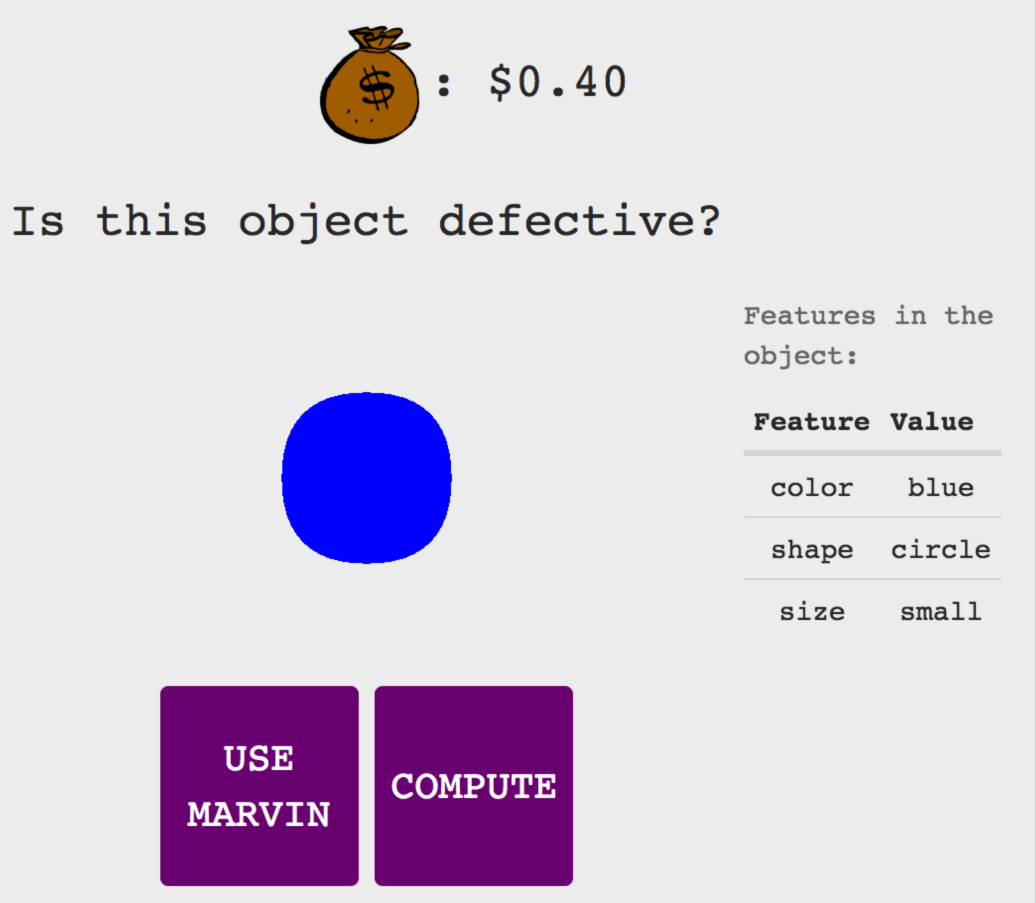
\includegraphics[width=0.8\linewidth]{tutorial-1.png}
    % \vspace{-0.2pc}
    \caption{Screenshot of the \plat\ platform for studying human-AI teams.}
    \label{fig:ui}
    % \vspace*{-1.0pc}
\end{figure}  

How might we study the impact of AI accuracy, updates, compatibility, and mental models on the performance of \name\ teams? Ideally, we would conduct user studies in real-world settings, varying parameters like the length of interaction, task and AI complexity, reward function, and the AI's behavior. All human-subjects research is challenging, but our setting poses special perplexities. Testing in real settings reduces or removes our ability to directly control the performance of the AI. Furthermore, it may largely measure experts' differing experience in the domain, rather than their interactions with the AI.
%Performance of a human-AI team is most directly affected by the problem-solving ability of the human.  If the human is an expert at the task, then the performance of the AI is unlikely to matter very much (except, perhaps, to speed the team), nor will the accuracy of the human's mental model. Most importantly, the {\em variability} in the level of human skill and problem-solving speed can significantly obfuscate other factors. 
%\Bug{WSL: we assume the human could be perfect in our study, but the efficiency comes from working as a team -- I think we should drop some of this content down-playing the importance in the case of an expert human (e.g., doctor)}
The importance of mental models for team success
%How central mental models are for team success 
varies among domains and the interaction designed between the AI system and humans. When humans do not have an easy way to validate machine correctness, extracting value out of AI assistance depends on the ability of the human developing a mental model of the AI system. 
%We considered tasks where humans were expert, yet the task was time consuming --- here, the AI could save the human decision-making time. But 

To control for human expertise and the centrality of mental modeling, we developed the \plat\ platform, which supports parameterized user studies in an assembly line domain that abstracts away the specifics of problem solving and focuses on understanding the effect of mental modeling on team success. \plat\ is designed such that {\em no} human is a task expert (nor can they become one). In fact, the true label of decision problems in the platform is randomly generated so that people cannot learn how to solve the task. However, humans can learn when their AI assistant, Marvin, succeeds and when Marvin errs. Alongside, the human has access to a perfect problem-solving mechanism, which she can use (at extra cost) when she does not trust Marvin. 

%However, conducting such studies is challenging, and more so than many other experiments with human subjects.  --- they require prolonged study periods, and they may be infeasible per risk of study in real-world settings and the difficulty of exploring combinations of parameters. To overcome these challenges, we develop a reusable platform to conduct studies in a simpler, abstract domain.

% Studying the performance of human-AI teams presents several challenges. As we describe in the problem setting, many of these challenges originate from the fact that human mental models might be imperfect and their quality hard to quantify. Moreover, in many real-world domains, it is not feasible to vary important parameters of the teamwork such as length of the interaction, task and model complexity, environment reward, or update compatibility. To facilitate research that explores settings in different combinations, we designed and developed an open-source  platform for conducting experiments in an abstract domain. The platform allows to investigate the effects of the following factors on team performance: (F1) task complexity, (F2) the complexity of the \emph{error boundary} of the classifier, (F3) reward, and (F4) AI updates. All these factors can be programmatically configured by the experimenter. 

Specifically, \plat\ is a web-based game, whose goal is to make classification decisions for a fixed number of box-like objects.  For each object, the team follows the steps S1-S4 to decide whether the object is ``defective" or not. In S1 a new object appears (\eg,\ blue square), in S2 the AI recommends a label (\eg,\ not-defective), in S3 the player chooses an action (\eg,\ accept or reject the AI recommendation), and in S4 the UI returns a reward and increments the game score. The objects are composed of many features, but only a subset of them are made {\em human-visible}.
% ;\Bug{\st{need to square this with subsequent language saying that the system behaves randomly BN: Included this in the paragraph above}}
For example, visual properties like shape, color, and size are visible, but the contents are not. In contrast, the AI has access to all the features but 
%has limited classification accuracy---it 
may make errors. At the beginning of the game, users have no mental model of the AI's error boundary. However, to achieve high scores, they must learn a model using feedback from step S4. Figure~\ref{fig:ui} shows a screenshot of the game at step S3. %\Bug{Marco: It's not clear if the user can see the model's prediction before accepting or not.  The screenshot seems to indicate the user can either trust the model blindly or make his own prediction. If this is the case, it's a little contrived. }

\plat\ allows study designers to vary parameters, such as the number of objects, number human-visible features, reward function, AI accuracy, and complexity of perfect mental model (number of clauses and literals in the   error boundary and stochasticity of errors). Further, it enables one to study the effects of updates to AI by allowing changes to these parameters at any time step. In the next section, we use \plat\ to answer various research questions.

% The platform is a Web-based game, where a human player is required to form a team with an AI named Marvin, and classify a fixed number of objects to achieve a high score. The classification task is to identify whether a box-like object-- composed of features such as shape, color, size, and inside contents-- is ``defective'' or not. Objects appear one-by-one, and for each object, the player must go through the steps S1-S4 to label it. 
% Since, in real-world domains, we may not have access to all the features, in the game, we hide some features from the user, \eg\ the inside contents of the object. The rest of the features are human-visible. Marvin, on the other hand, gets access to all the available features but has limited classification accuracy. The correct label depends on all the features, so to perform well, at step S3, the player must decide when to rely on Marvin by creating a mental model of it.

% Figure~\ref{fig:ui} shows a screenshot of the game at step S3. 
% The reward function is defined as a matrix. Table~\ref{tab:payoff} shows an example of the reward matrix used in the user studies describe in the Experiments section.
% The platform allows varying various factors in teamwork: length on interaction, task complexity, complexity of the AI, human-visible features,
%  updates, accuracy of AI, shape of the error boundary.
% In the experimental section, we vary these parameters to answer various research questions. 
% While for brevity we do not exhaustively present results from the whole experimental spectrum, the goal of the platform is to enable further studies in the same vein.
% The web-based user interface of the platform implements an assembly line game where the goal of the team is to identify whether a box-like object on the assembly line is ``faulty'' or not. Each object has various features (\emph{e.g.}, shape, color, size, content etc.) as well as a ground truth label (\emph{faulty} or \emph{non-faulty}). The  label of the object depends on the complete feature set, which is not fully observable by the human (\emph{e.g.}, the content of the object). Therefore, the user can create a mental model of when to trust the classifier only based on the human-visible features.

% The game contains $T$ cycles and in each cycle:
% \begin{itemize}
%     \item[S1] A new object appears (\emph{e.g.}, a blue square) and the user sees all the human-visible features.
%     \item[S2] AI makes a prediction based on all the features. 
%     \item[S3] The player decides whether to accept or compute the label. 
%     \item[S4] The UI returns a reward based on the reward matrix.
% \end{itemize}

% Figure~\ref{fig:ui} shows a screenshot of the game at step S3. At the end of the interaction, the final score of the team is computed as the sum of rewards $R$. For each interaction, the experimenter can decide whether to introduce an AI update at a given time step $t_{update}$, and whether to notify users about this event.



% For this game, the platform allows varying the various factors mentioned earlier as follows. Task complexity (F1), is expressed by the number of human-visible features. For example, in Figure~\ref{fig:ui}, one can add more visual properties to show to the user, such as size and texture. The complexity of the model's \emph{error-boundary} (F2) is shown by the complexity and the stochasticity of feature space regions where the AI errs. We specify these regions as a First-Order Logic (FOL) formula with clauses and literals (\emph{e.g.}, $blue \cap square$). Complexity can be varied by adding more literals and clauses (\emph{e.g.}, $(blue \cap square) \cup (red \cap circle \cap checkered)$). These regions can be configured to be fully deterministic (\emph{e.g.}, the classifier errs for all $blue \cap square$ objects) or stochastic (\emph{e.g.}, the classifier errs for 90\% of $blue \cap square$ objects). Stochastic error regions are useful for studying cases where the complete feature set is larger than the human-visible feature set and certain classifier predictions might appear as stochastic to users since they only have a partial view of features.

% Reward (F3) can be configured in a matrix form as shown in Table~\ref{tab:reward_matrix}, assigning  custom rewards and penalties to different team outcomes. For example, if the goal is to design a high-stake game, $r(0,1)$ should be negative and higher in absolute value compared to the other matrix entries. If in contrary, the cost of human inspection is high, the reward for inspected cases (\emph{i.e.}, $r(1,0)$ and $r(0,0)$) should be lower than for cases when the user correctly trusts a classifier (\emph{i.e.}, $r(1,1)$). Note that, in the current reward formulation, we indirectly assume that human inspection will predict the correct label. Although this might not always be the case, this design choice was made to study the impact of mental models on the success of AI updates decoupled from the problem of human problem-solving skills. In future work, we see important developments ahead for jointly studying these problems, especially for forms of human-AI interaction other than HCAI.   

% Finally, in order to customize properties of the AI update, the platform supports changing the accuracy of the updated model as well as the shape of the new error boundary with respect to the original one. To this end, it is possible to experiment four types of update settings: (i) \emph{no update} does not change either the AI accuracy or its error boundary (ii) \emph{no change} preserves exactly the same error boundary but the AI accuracy increases, (iii) \emph{subset} increases accuracy and the error boundary is compatible, \emph{i.e.}, does not introduce new errors, (iv) \emph{no intersection} increases accuracy but the error boundary is incompatible, \emph{i.e.}, it introduces new errors.

% In the experimental section, we show representative findings from human studies examining the role of these factors. While for brevity we do not exhaustively present results from the whole experimental spectrum, the goal of the platform is to enable further studies in the same vein.

% Platform is a human facing UI
%     - human and AI work as a team to solve a shared classification task 
% Follows interaction pattern described in last section
% simulates long-terms repeat interaction between team members
% UI implements an assembly line-like game
% objects with various visual properties appear one-by-one
% the task is find the objects with the true label "faulty"
% the game contains N rounds
% In each round:
%     - A new object arrives e.g., blue square (human-visible features)
%     - AI makes a prediction using all (AI-visible features)
%     - Based on human-visible features, user decides whether to trust AI or override
%     - Figure shows a screen shot after step 2 [Add: zoomed in screenshot of UI like the one in instructions]
% Factor->mechanism:
% a Complexity of task->number of human-visible features
% b Complexity of error boundary->
%     make errors on c, vary number of clauses and literals in c
%     b stochasticity vary p(err | c), 
% c updates -> improve accuracy, change errors: no-change, subset, mutually exclusive


% \begin{figure}[H]
%     \centering
%     \includegraphics[width=\linewidth]{4.pdf}
%     \caption{Performance deteriorates after update step.}
%     \label{fig:updateExp2}
% \end{figure}


% 0
% study with mturk workers
% X workers per observation
% average hourly wage: 
% removed the bottom 25\% for each setting
% a better mental model should lead to higher team performance

% [Add: Single plot with three sub-figures, one for each bullet]


% \vspace{-2mm}
\section{Experiments}
We present experiments and results in two parts. First, using our platform, we conduct user studies to understand the impact of mental models and updates on team performance. Second, we simulate updates for three real-world, high-stakes domains and show how the retraining objective enables an explorable tradeoff between compatibility and performance that is not available in the original models.


%\begin{itemize}
%    \item[Q1.] Does a better mental model of AI lead to higher team performance? (Figure~\ref{fig:wsl})
%    \item[Q2.] How do the complexity of task and the AI affect a user's ability to create a mental model? (Figure~\ref{fig:nonStochasticExp})
%    \item[Q3.] Does a more compatible update lead to higher team performance than incompatible update? (Figure~\ref{fig:updateExp}) \Bug{This result also appeared before in 3.1, change the statement} 
%    \item[Q4.] Do the current ML pipelines produce highly compatible updates? (Table.~\ref{tab:score})
%    \item[Q5.] Does there exists a trade-off between performance of AI and its compatibility? (Figure~\ref{fig:trade-off})
%    \item[Q6.] What is the relative performance of different dissonance functions? (Figure~\ref{fig:diss})
%\end{itemize}

%\subsection{User Studies}
% \vspace{0.1pc}
\noindent {\bfseries User Studies.} In user studies, we hired MTurk workers and directed them to the \plat\ platform.\footnote{Workers were paid on average \$20/hr, over the minimum wage in line with  ethical guidelines for requesters~\cite{dynamo-MT-ethics17}.} We informed them of the purpose of the study and provided a set of simple instructions to familiarize them with the task and the user interface: form a team with an AI, named Marvin, and label a set of 100 objects as ``defective'' or ``not defective''.  
% \Bug{\st{need to say how much we paid workers and effective hourly wage; ideally cite something saying that this is ethical like "which is in accordance with Mechanical Turk guidelines for academic requesters~\cite{dynamo-MT-ethics17}}} 
Following \name, to label an object, a worker can either accept Marvin's recommendation, which is initially correct 80\% of the time, or use the ``compute'' option, which is a surrogate for the human doing the task herself perfectly but incurring an opportunity cost.
Table~\ref{tab:payoff} summarizes the reward function  used in our studies. The matrix is designed in a way that it imitates a high-stakes scenario, i.e., the monetary penalty for a wrong decision is much higher than the reward for a correct decision. We found this design choice to be a good incentive for workers to learn and update their mental model on Marvin.  %;  mistakes incur a high penalty, as is typical in high-stakes domains.  ``Computing'' yields a uniform reward of zero, which results from the an increased cost to the human counterbalanced by never making a mistake.  
Note that the expected value of a pure strategy (\eg, always ``Compute"  or always ``Accept," without considering the likelihood of Marvin's correctness) is zero. The only way to get a higher score is by learning when to trust Marvin. While the subjects are told  Marvin's accuracy and the payoff matrix, they can only learn Marvin's error boundary gradually by playing the game.   These design choices allow us to study the impact of mental models while controlling for human problem solving expertise --- every player is able to solve  problems perfectly, at a fixed cost,  using ``compute.''\\

% As noted in the platform description, the true labels are randomly generated and so the human can't solve the problem except by trusting Marvin or using ``compute.''  by design can not see Marvin's recommendation, which would be an unhelpful distraction.g

%Conceptually, ``computing'' never makes mistakes but takes is always right but yields zero reward.  As noted in the platform description,  the true labels are randomly generated and workers by design can not see Marvin's recommendation, which would be an unhelpful distraction. These design choices allow us to study the impact of mental models in isolation of human expertise at problem solving. %In the same line of thought, clicking the `Compute" button automatically submits the correct answer. 


% \Bug{\st{Move the text to platform .; Introduce controlling for human expertise? BN: I am putting a few lines here but expecting that there should be changes in the platform too}}

%However, there is a challenge: If we make it easy to compute the correct label, then workers can complete the task without help from Marvin and without learning the error boundary. To prevent this, we assign the correct labels using a random function, and hide Marvin's recommendations so that they cannot learn the task indirectly. Also, to simplify the setup, we assume that workers are perfect; the UI submits the correct label if a worker clicks on the ``Compute" button. 

% All user studies were conducted on Amazon Mechanical Turk by presenting to workers specified instances of the assembly line game.
% The classification task is to predict whether an object is ``faulty''.
% Objects appear one-by-one for 100 cycles. They are composed of a maximum of six binary features including shape, color, size, and texture. We assign true labels to objects using a random function so that it is harder for participants to learn how to do the task by themselves. Again, this configuration choice was introduced to study the impact of mental models independently from how well participants can learn how to solve the classification task. For the same reason, we assume that all human inspections during the game override the AI prediction with the true label. This is also reflected in the reward function used in the game as shown in Table~\ref{tab:payoff}. According to the above assumption, the exact reward of inspection would be computed by subtracting the cost of inspection from the reward of making a correct prediction. This would assign the same reward to all inspection cases. In order to make the reward function easier to understand for crowdsourcing workers and fair at the same time, we assign a zero reward for both inspection cases and equally increase the reward for the acceptance column. \footnote{Workers earned on average an hourly wage of \$20/hr.} In addition, the reward function imitates a high-stakes domains by assigning a highly negative reward to acceptances of wrong AI recommendations. 


% Even though we assign the true labels randomly, we keep the error boundary simple: it can be expressed as a FOL formula $f$ in disjunctive normal form, where literals are features, \eg, $f = blue \cap square$. 

%The cumulative of this reward is a measure of the team's performance.\Bug{This sentence does not belong here. The problem setting should say this.}

\begin{table}[t]
    \centering
    \begin{tabular}{|c|c|c|}
    \hline
         & Accept & Compute  \\
         \hline
         AI right & \$0.04 & 0 \\
         \hline
         AI wrong & -\$0.16 & 0\\
         \hline
    \end{tabular}
    \caption{Reward matrix for the user studies. To mimic high-stakes domains, penalty for mistakes is set to high. 
    %If a worker inspects, she always submits a correct prediction and gets a reward of 0. However, if she accepts the AI's recommendation, she can either earn \$0.04 or lose \$0.16 depending on whether the recommendation was right or wrong.
    }
    \label{tab:payoff}
\end{table}


\begin{figure*}[t]
  \centering
%   \begin{subfigure}[b]{.45\columnwidth}
%     \centering
%     \includegraphics[width=\columnwidth]{payoff.png}
%     \caption{}
%     % \caption{Team performance vs. complexity of task/error boundary. Performance drops for complex tasks and error boundaries.}
%   \end{subfigure}
%  \hfill 
  \begin{subfigure}[b]{.47\columnwidth}
    \centering
    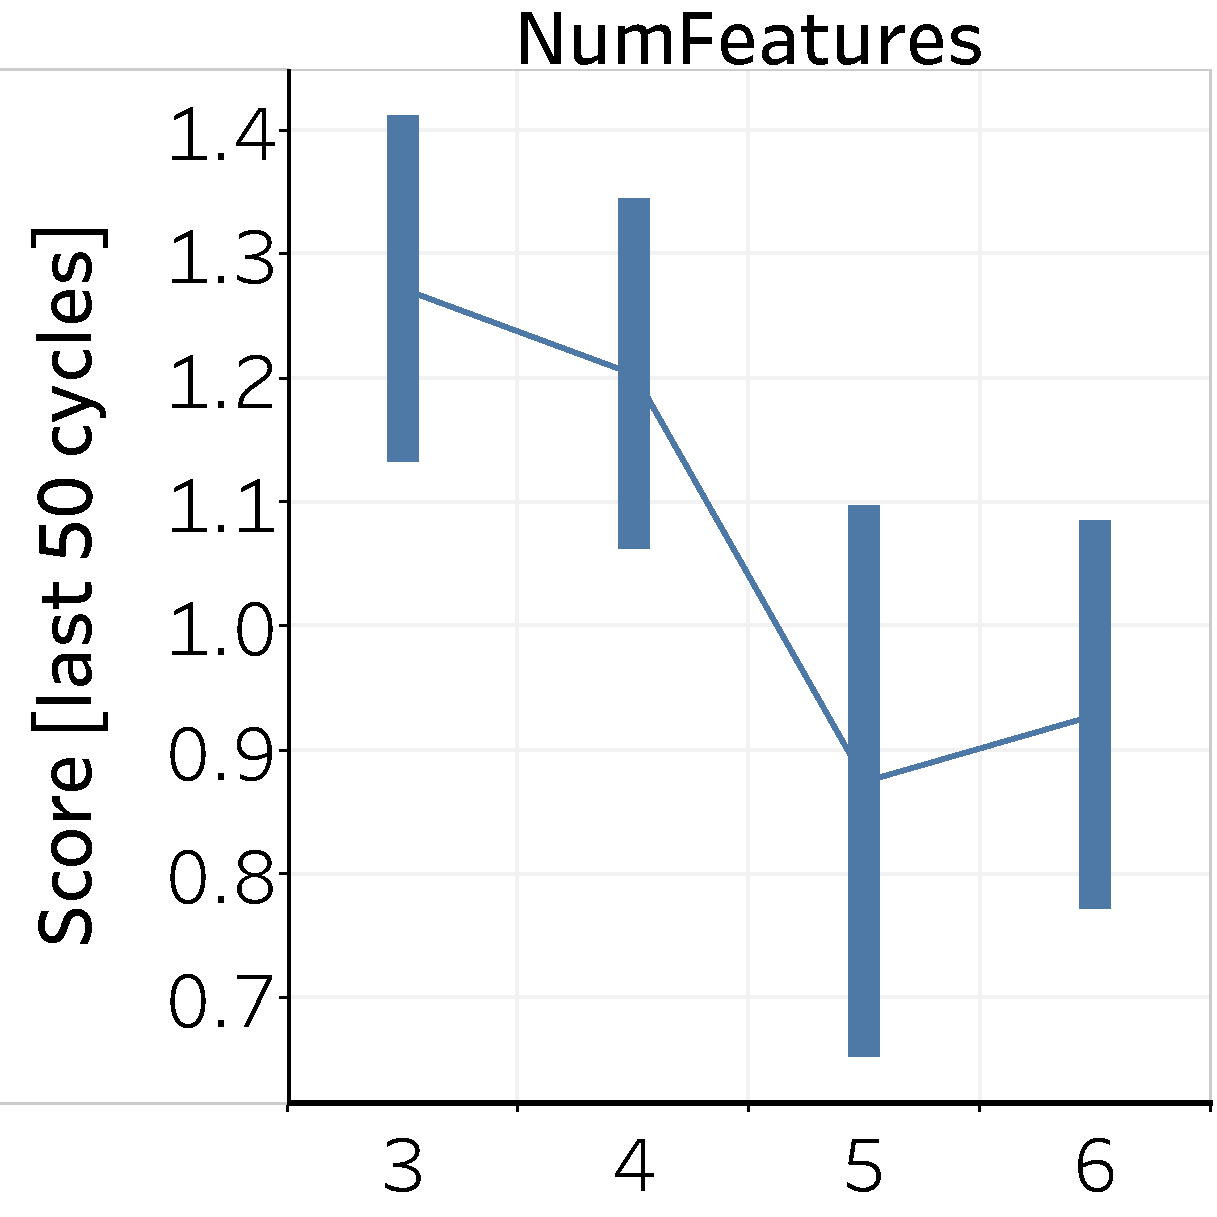
\includegraphics[width=\columnwidth]{2a.pdf}
    \caption{}
    % \caption{Team performance vs. complexity of task/error boundary. Performance drops for complex tasks and error boundaries.}
    \label{fig:complexity_nonstochastic}
  \end{subfigure}
  \hfill
  \begin{subfigure}[b]{.47\columnwidth}
  \centering
    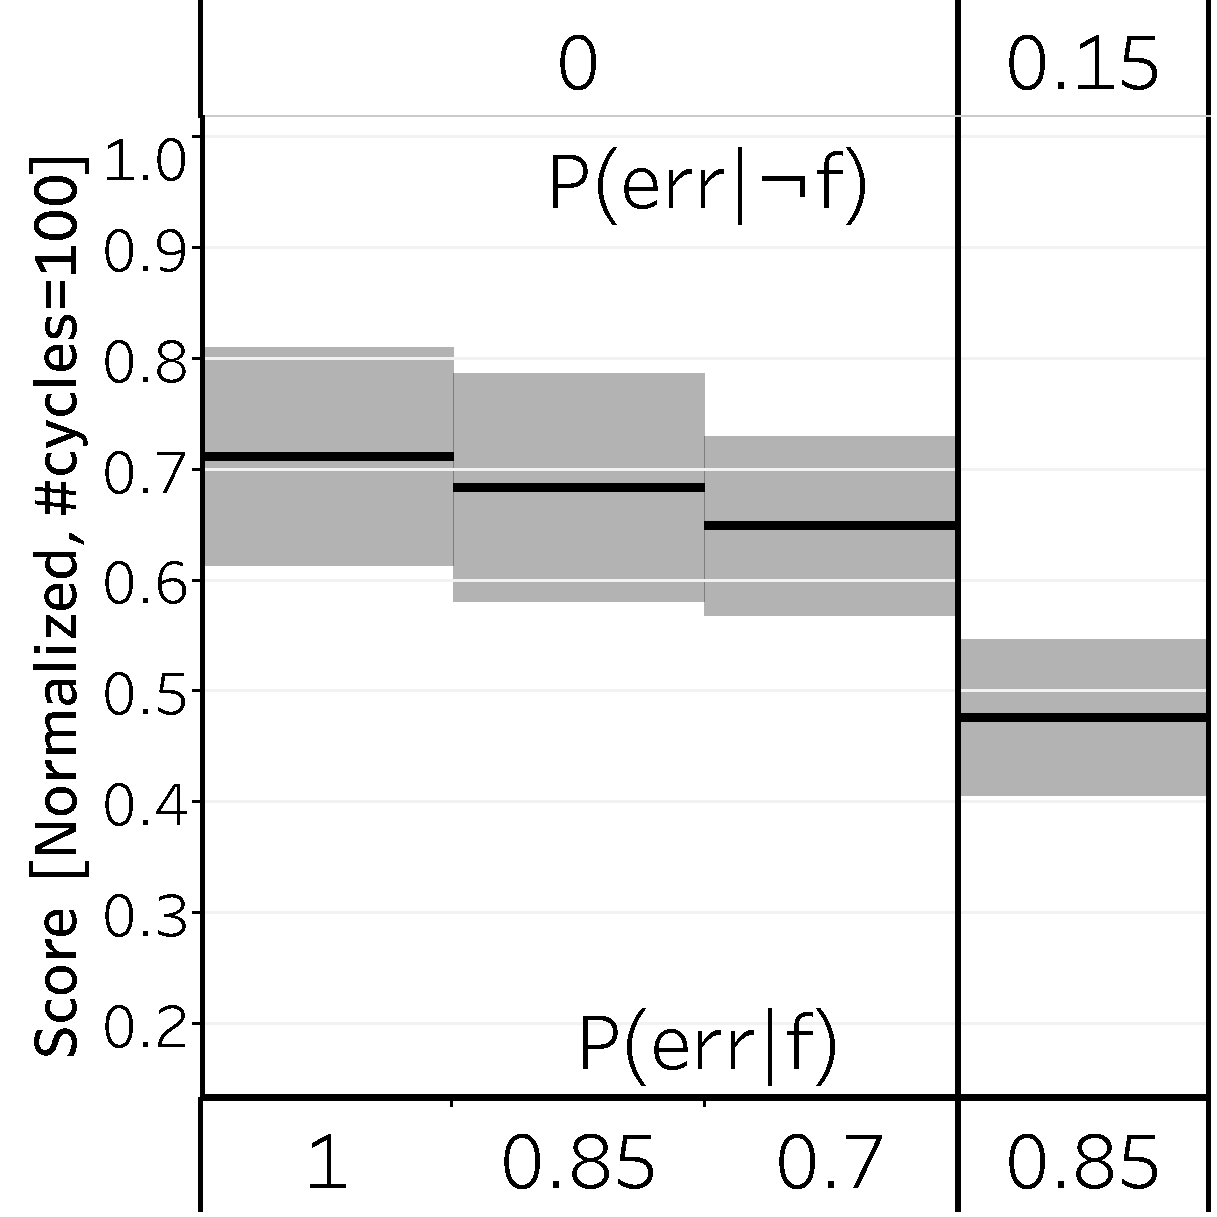
\includegraphics[width=\columnwidth]{2b.pdf}
    \caption{}
    % \caption{Team performance vs. stochasticity. 
    % %The left pane shows results for one-sided errors, while the right pane focuses on two-sided errors.
    % Performance drops for more stochastic/complex error boundaries. The Y-axis indicates a raw normalized with the performance of the optimal policy. We normalize because when we vary stochasticity, the optimal policy in the different conditions may score differently.}
    \label{fig:complexity_stochastic}
  \end{subfigure}
    \hfill
  \begin{subfigure}[b]{0.47\columnwidth}
  \centering
    \centering
    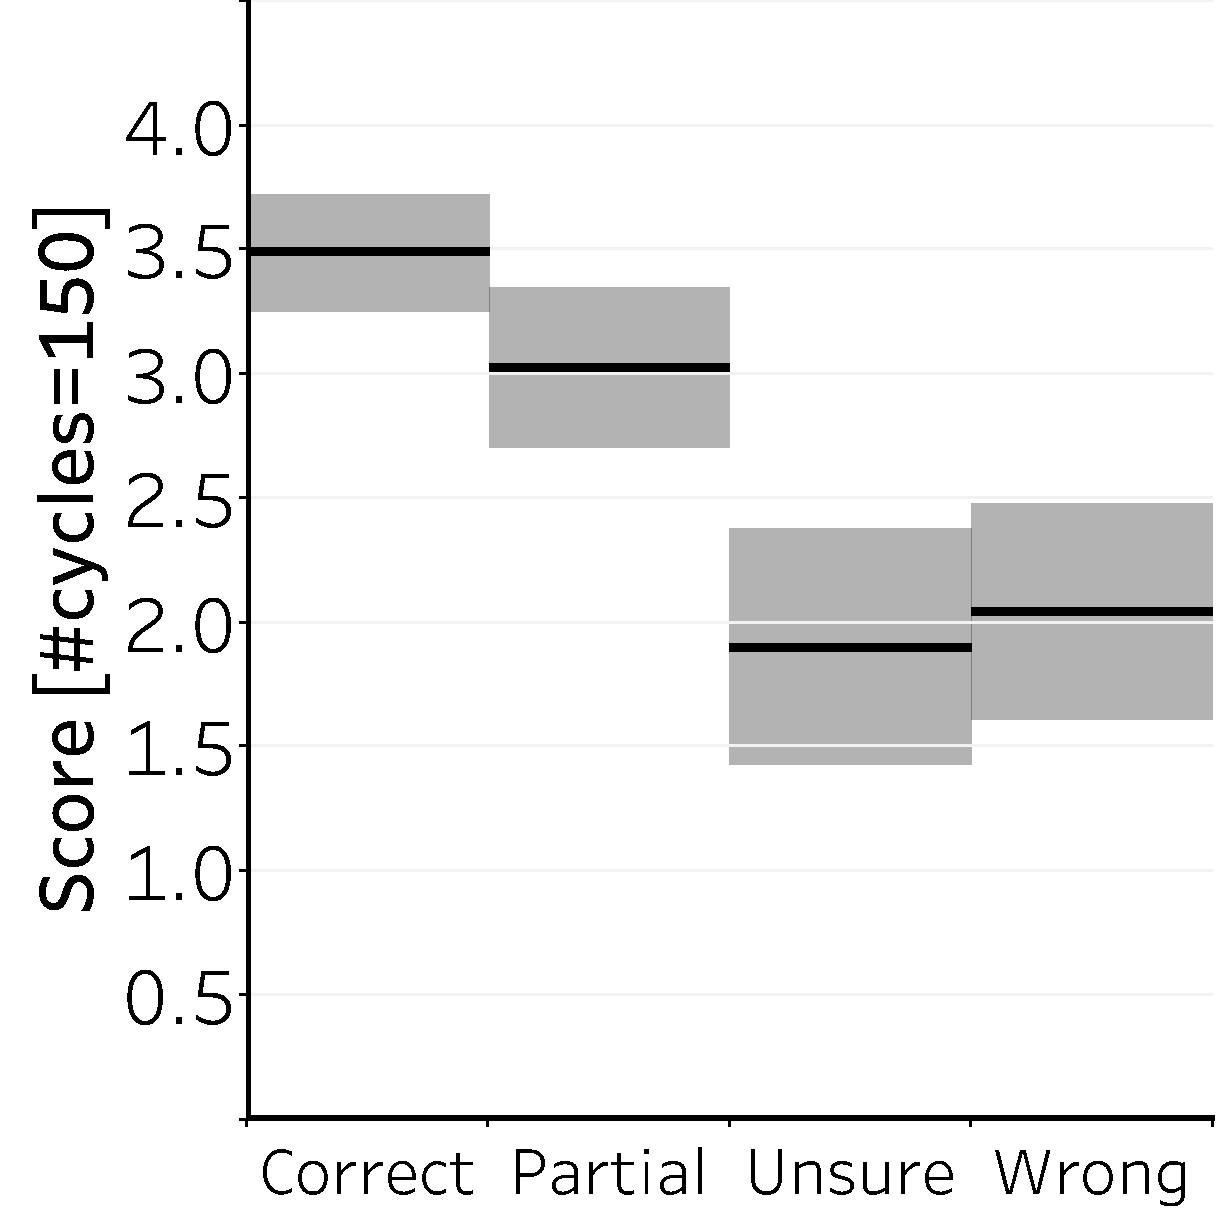
\includegraphics[width=\columnwidth]{wsl.pdf}
    \caption{}
    % \caption{Team performance vs. mental model quality. Wrong/unsure mental models result in lower performance.}
    \label{fig:wsl}
  \end{subfigure}
  
  \caption{(a) Team performance decreases as we increase the number of human-visible features. (b) Team performance decreases with the stochasticity of errors. The decrease is much higher for two-sided errors. (c) Better mental models result in higher team performance. Wrong and Unsure mental models have the lowest performance. 
  }
  \label{fig:complexity}
\end{figure*}
% \Bug{BN: 1) If we decide to remove the 1c3l and 2c2cl conditions, we need to remove them from the platform description too, as they're not relevant anymore. 2) As a future reference, I don't think we should not be super uncomfortable with the fact that some conditions intersect with each other (1c2l vs 2c2l). These are human studies and humans are not all alike. Some might find certain conditions easier than others. Also some might put more attention to more difficult tasks and perform even better. If one could control for both these (skills and focus), then yes, probably non-intersecting results could be possible.}

\begin{figure}[t]
  \centering
    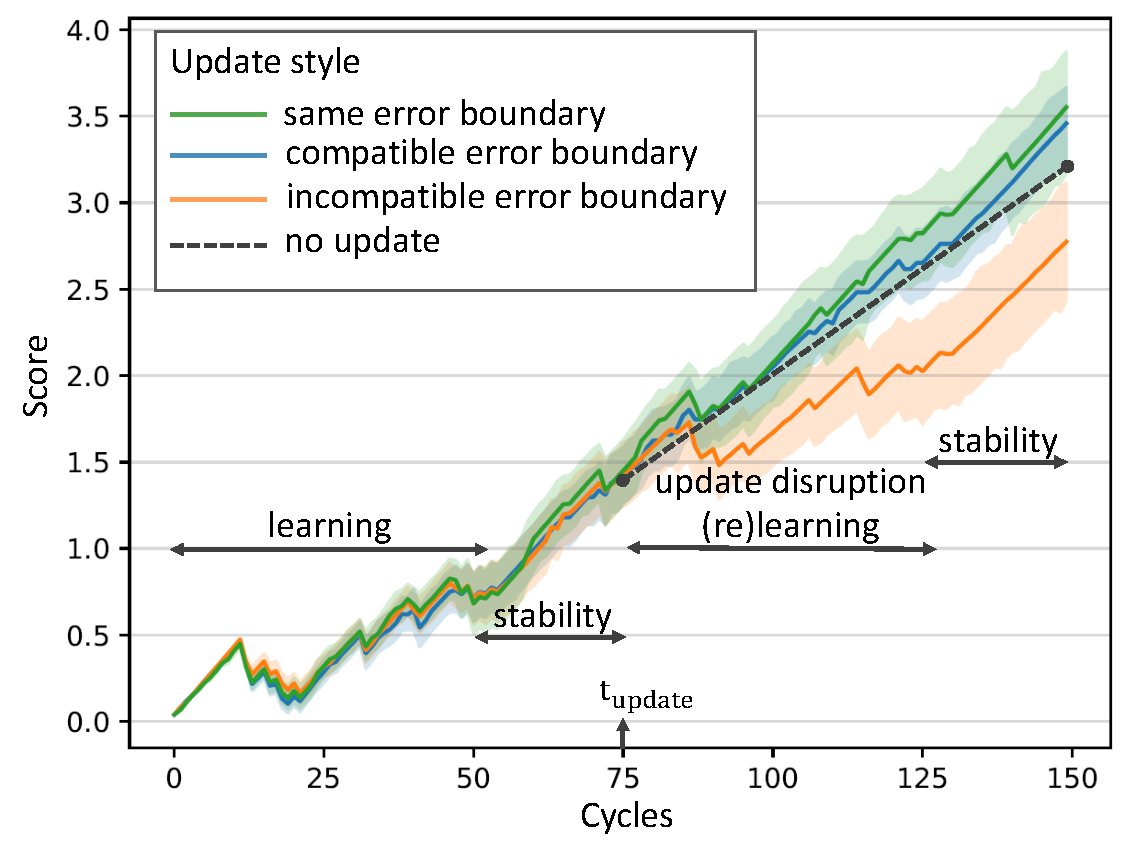
\includegraphics[width=\columnwidth]{update_study.pdf}
    \caption{Team performance for different update settings. Compatible updates improve team performance, while incompatible updates hurt team performance  despite improvements in AI accuracy.}
    % \caption{Team performance for different update settings. Compatible (subset) updates guarantee team improvements.
    % %TODO: Update study, pvalue between col 1 and 3 = 0.001, pvalue between 1 and 2 = 0.85. Between dotted and col 3 = 0.1
    % }
    \label{fig:updateExp}
\end{figure}

%\noindent {\bfseries Q1: }{\em How do the complexity of the task and the error boundary affect the human ability to create a mental model?}
\noindent {\bfseries Q1: }{\em Do better mental models of AI lead to higher team performance?}\\
\noindent To answer this, we conducted human studies that measured team performance across different conditions of complexity of task and error boundary.
For each condition, we hired 25 MTurk workers, and filtered spammers by deleting data from workers in the bottom quartile.  
We varied the task complexity by varying the number of human-visible features. The complexity of error boundary $f$, expressed as a logical formula, is varied by changing the number of conjuncts and literals in $f$. For example, we tried one conjuncts containing two literals, one conjunct with three literals, and two conjuncts with two literals. 
Since many features can be used as literals,  we chose them randomly to create different but isomorphic error boundaries. For example, worker A gets $f_A = (blue \cap square)$ and worker B gets $f_B = (red \cap circle)$.
Figure~\ref{fig:complexity_nonstochastic} shows that, for one conjunct and two literals, team performance decreases with the number of features. We observed a similar behavior for other error boundaries (results omitted for space), and for the rest of these studies we set the number of conjuncts to one.
 Figure~\ref{fig:complexity_nonstochastic} shows that, as the number of features increases, team performance decreases because it becomes harder to create a mental model.
% In summary, we observe that teamwork is more efficient in less complex conditions mapping to better mental models.
%, as well as the number of literals and clauses in the error boundary $f$ to control its complexity. We experiment with three {\em types} of formulas: a single conjunction with two literals (1c2l), a single conjunction with three literals (1c3l), and two conjunctions of two literals (2c2l).  Similarly, the team performance is much lower for complex error boundaries (2c2l) than for simpler ones (1c2l). Here, the classifier's accuracy is fixed to 0.8 and 25 workers play the game for each condition. 

Next, we conducted a study (Figure~\ref{fig:complexity_stochastic}) to understand the impact of {\em stochasticity} in the error boundary on team performance.  
Stochasticity is defined using two conditional probabilities: $P(\err | f)$ and $P(\err | \neg f)$. That is, the probability of error if $f$ is satisfied, and if it is not satisfied. To vary stochasticity, we chose the following four pairs of probabilities: (0.7, 0), (0.85, 0), (1.0, 0), and (0.85, 0.15). For the first three pairs, the errors are ``one-sided'': since $P(\err|\neg f)$ is 0, the classifier makes a mistake only if the formula is satisfied. In the last pair, errors are ``two-sided'': with a probability of 0.15, the classifier makes a mistake even if the formula is not satisfied.
We fix the number of features to three and the number of literals to two.
Figure~\ref{fig:complexity_stochastic} shows that as errors become more stochastic, it becomes harder to create a mental model, deteriorating team performance. The $y$-axis shows the score normalized by the score of the optimal policy because, as we vary stochasticity, the optimal policy's score changes.

Finally, in order to have a closer view of the quality of the workers' mental models, we ask them to self report when they thought Marvin was wrong. We manually labeled these reports as correct, partial, unsure, and wrong, without looking at their team performance. The label denotes how the worker's mental model compared to the true error boundary $f$. For example, correct denotes that the mental model and $f$ were the same, wrong denotes no match, partial denotes an incomplete match, and unsure denotes that the worker was skeptical of their mental model. Figure~\ref{fig:wsl} compares team performance on these groups. Workers with the correct mental model score the highest, followed by workers with a partially correct model. These observations confirm that better mental models contribute positively to team performance.\\




% - For F1 and F2, we describe two user studies: M x N study, P x Q study.
% - first study varies number of features and complexity of error boundary. observations apply to F1 and F2
%         - we vary from 3-6
%         - change number of literals and clauses: 1c2l, 1c3l, 2c2l
% - in second study, we fix number of features and complexity of error boundary, but vary the ``stochasticty'' of errors. observations apply to F2.
%     - change stochasticity: 
%         - one-sided: p(err|notc) is 0, p(err|c) is 0.7, 0.85, 1. 
%         - two-sided errors: p(err|c)=0.85, p(err|notc)=0.15 
% - Figure~\ref{fig:nonStochasticExp}


\noindent {\bfseries Q2: }{\em Do more compatible updates lead to higher team performance than incompatible updates?}\\
% \Bug{Do we need acronyms?}
\noindent To study the impact of updates, we set the number of cycles to 150, and at the 75th cycle, update the classifier to a version that is 5\% more accurate (80\% $\rightarrow$ 85\%). Then, we divide the participants into three groups: same error boundary,
% \Bug{still very confusing that no change means there was a change!  I understand that you want a shorter name than 'incompatible error boundary' but what about calling the conditions SEB, CEB and IEB -- put these ackronyms in the figure and use them here instead of subset etc?}
compatible error boundary, and incompatible error boundary. The same error boundary group receives an update improving accuracy, but the  error boundary is unchanged. For the two other groups, the number of literals (features) in the error boundary changes from two to three. The update for the compatible error boundary group introduces no new errors; for example, if before the update the error boundary was $blue \cap square$, after the update it may change to $small \cap blue \cap square$. For the incompatible error boundary group, the error boundary introduces new errors violating compatibility. Figure~\ref{fig:updateExp} summarizes our results. We also show the performance of workers if no update was introduced (dashed line). It uses the no-update setting from experiments in Q1, and extrapolates from there assuming that the worker's mental model is already stable at the 75th cycle, meaning that the human-AI team has reached the maximum performance for the original setting and no further improvements are expected. The graph demonstrates two main findings on the importance of compatibility. First, a more accurate but incompatible classifier  results in lower team performance than a less accurate but compatible classifier (no update). Second, compatible updates improve team performance. Moreover, the figure shows different stages during the interaction: the user learning the original error boundary, team stabilizes, update causes disruption, and performance stabilizes again. A central insight in the update stage is that the incompatible error boundary condition sacrifices the team score while workers have to relearn the new boundary. This insight shows that compatible updates not only improve team performance but they can also reduce the cost of retraining users after deploying system updates.  
%Participants were divided into four groups: no update, no change, subset, and no intersection. The no-update group never receives an update, and the no-change group receives an update, but it does not change the error boundary.
%The update for the subset group introduces no new errors: if before the update the error boundary was $blue \cap square$, after the %update it may change to $small \cap blue \cap square$. For the no-intersection group, the error boundary introduces new errors violating compatibility. Figure~\ref{fig:updateExp} summarizes results from this study. 
%It highlights two findings on the importance of compatibility. First, a more accurate but incompatible classifier (no intersection) results in lower team performance than a less accurate but compatible classifier (no update). Second, compatible updates (subset) improve team performance. 

%\begin{figure}[t]
%    \centering
%    \includegraphics[width=.65\columnwidth]{2c.pdf}
%    \caption{Team performance for different update settings. Compatible (subset) updates guarantee team improvements.
    %TODO: Update study, pvalue between col 1 and 3 = 0.001, pvalue between 1 and 2 = 0.85. Between dotted and col 3 = 0.1
%    }
%    \label{fig:updateExp}
%\Bug{Change figure to include results from the notify conditions}
%\end{figure}   
% \Bug{Change wording so that first column is the dotted line}

%\begin{figure}[t]
%    \centering
%    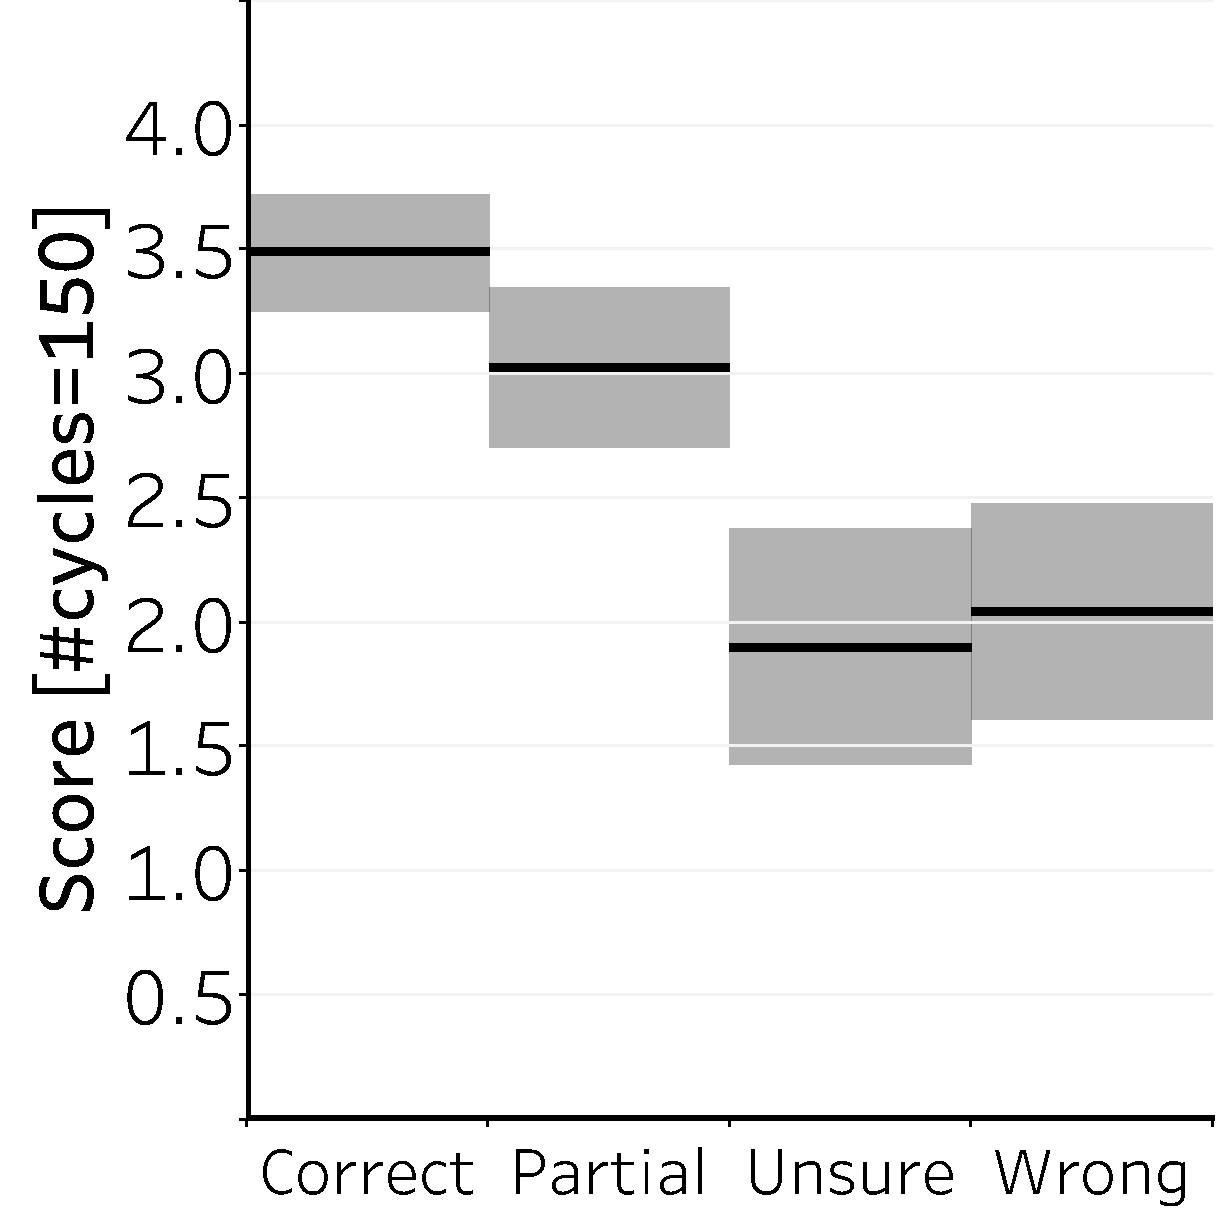
\includegraphics[width=.56\linewidth]{wsl.pdf}
%    \caption{Team performance vs. mental model quality. Wrong/unsure mental models result in lower performance.}
%    \label{fig:wsl}
%\end{figure}

\subsection{Experiments with  High-Stakes Domains}
\noindent {\bfseries Datasets.} To investigate whether a tradeoff exists between  performance and compatibility of an update, we simulate updates to classifiers for three domains: recidivism prediction (Will a convict commit another crime?)\cite{angwin2016machine}, in-hospital mortality prediction (Will a patient die in the hospital?) \cite{johnson2016mimic,harutyunyan2017multitask}, and credit risk assessment (Will a borrower fail to pay back?)\footnote{\url{https://community.fico.com/s/explainable-machine-learning-challenge}}. We selected these high-stakes domains to highlight the potential cost of mistakes caused by incompatible updates in human-AI teams.\\\\

\begin{table}[t]
\footnotesize
\centering
\begin{tabular}{|l|l|c|c|c|}
\hline
Classifier & Dataset                         & ROC $\hone$ & ROC $\htwo$ & $\compatscore(\hone, \htwo)$ \\
\hline
LR & Recidivism       &   0.68 &        0.72     &   0.72               \\
& Credit Risk          &   0.72     &    0.77    &   0.66              \\
& Mortality    &    0.68 &    0.77    &    {\bf 0.40}                    \\
\hline
MLP & Recidivism   &   0.59     &     0.73   &     0.53                    \\
& Credit Risk     &  0.70   &    0.80    &     0.63                     \\
& Mortality &       0.71 &     0.84   &     0.76            \\
\hline
\end{tabular}
% \vspace*{-0.5pc}
\caption{\label{tab:score} Although training on a superset of data increases classifier performance, compatability can be suprisingly low.}
%\caption{\label{tab:score} Performance and compatibility of ML classifiers.}
% \vspace*{-1.2pc}
\end{table}


\begin{figure*}[t]
    \centering
    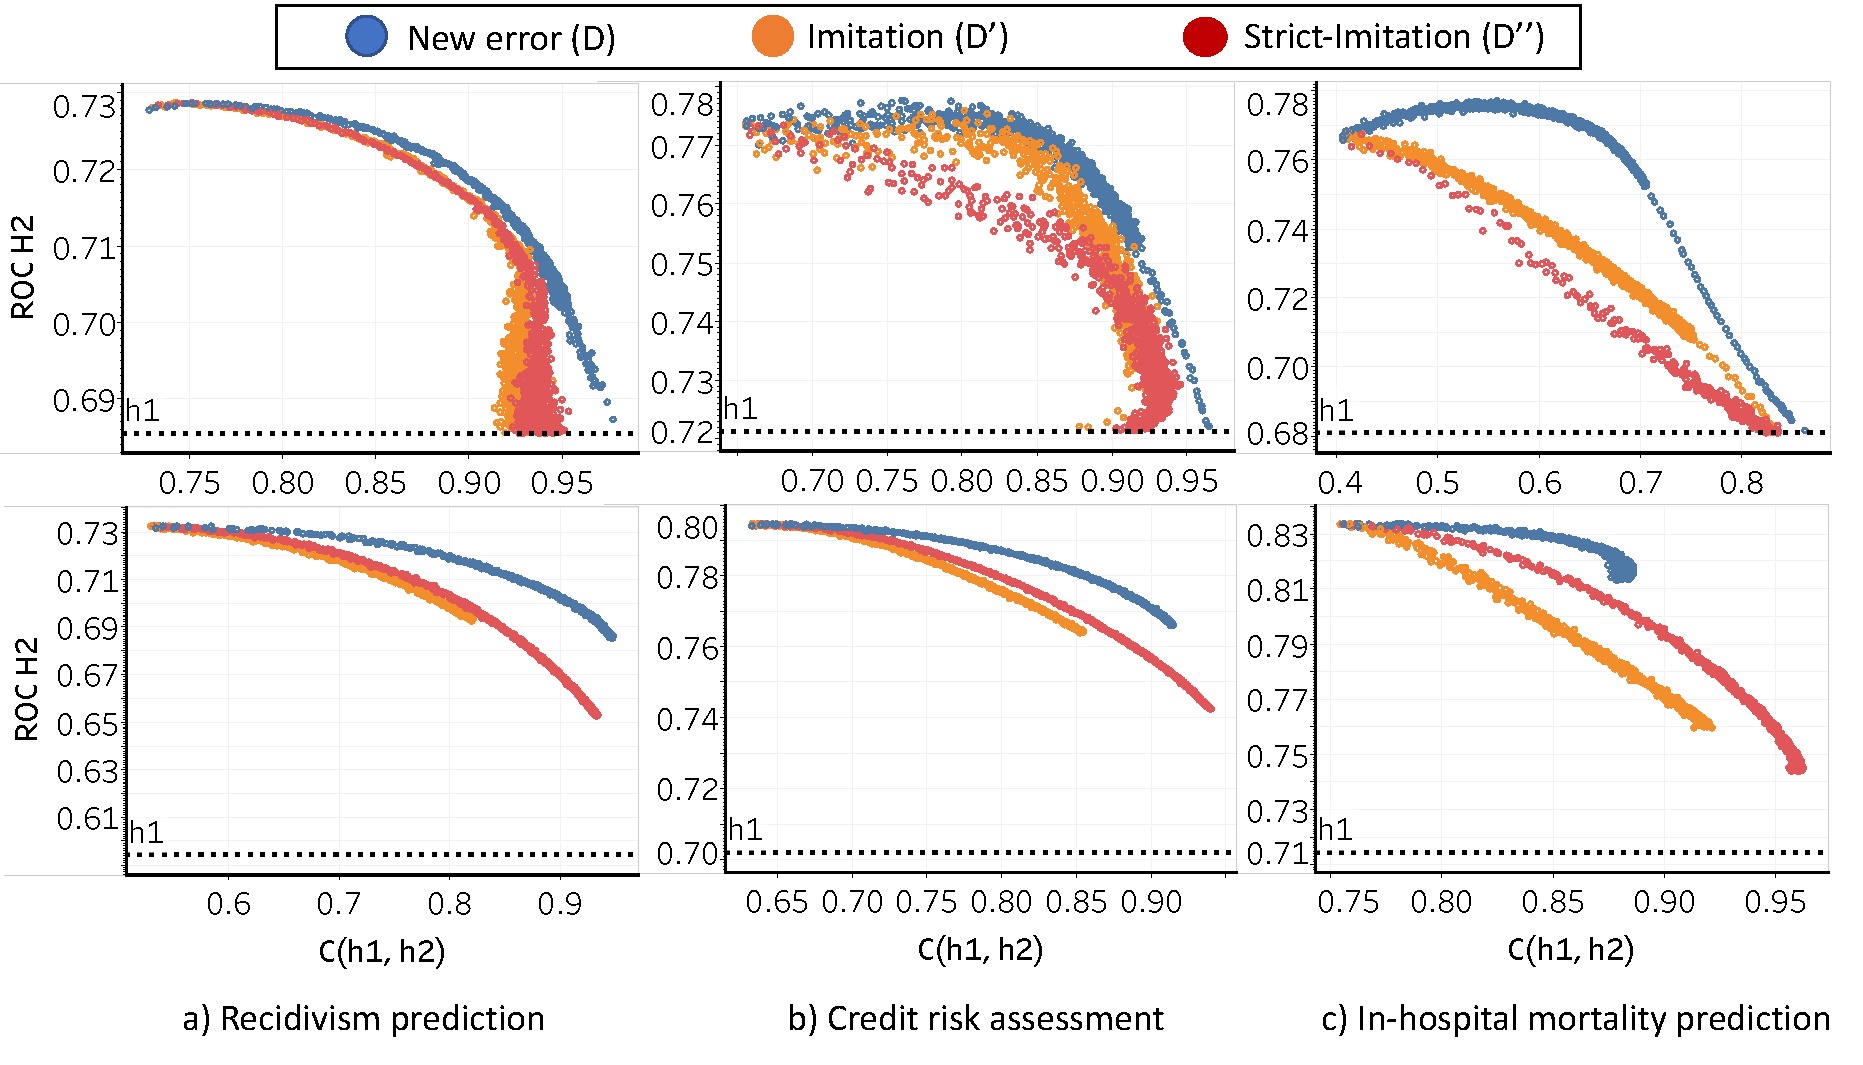
\includegraphics[width=0.9\linewidth]{figure5.pdf}
    %\vspace{-0.6em}
    \caption{Performance vs. compatibility for a logistic regression and multi-layered perceptron classifiers. The reformulated training objective ($\lossbc$) offers an explorable performance/compatibility tradeoff, generally more forgiving during the first half of the curves. The training objective based on new-error dissonance performs the best, whereas the ones based on imitiation and strict-imitation dissonance perform worse since they imitate probabilities of a less accurate, and less calibrated model ($\hone$).}
    \label{fig:diss}
\end{figure*}
% \begin{subfigure}{0.32\linewidth}
%     \includegraphics[width=\linewidth]{recid_logistic.pdf}
%     % \vspace*{-1.0pc}
%     \caption{Recidivism Prediction}
% \end{subfigure}
% \begin{subfigure}{0.32\linewidth}
%     \includegraphics[width=\linewidth]{fico_logistic.pdf}
%     % \vspace*{-1.0pc}
%     \caption{Credit Risk Assessment}
% \end{subfigure}
% \begin{subfigure}{0.32\linewidth}
%     \includegraphics[width=\linewidth]{mortality_logistic.pdf}
%     % \vspace*{-1.0pc}
%     \caption{In-Hospital Mortality Prediction}
% \end{subfigure}
% \begin{subfigure}{0.32\linewidth}
%     \includegraphics[width=\linewidth]{recid_mlp.pdf}
%     % \vspace*{-1.0pc}
%     \caption{Recidivism Prediction}
% \end{subfigure}
% \begin{subfigure}{0.32\linewidth}
%     \includegraphics[width=\linewidth]{fico_mlp.pdf}
%     % \vspace*{-1.0pc}
%     \caption{Credit Risk Assessment}
% \end{subfigure}
% \begin{subfigure}{0.32\linewidth}
%     \includegraphics[width=\linewidth]{mortality_mlp.pdf}
%     % \vspace*{-1.0pc}
%     \caption{In-Hospital Mortality Prediction}
% \end{subfigure}
% \Bug{Fig 3b change }
% \begin{subfigure}{0.32\linewidth}
%     \includegraphics[width=\linewidth]{recid_mlp.pdf}
% \end{subfigure}
% \begin{subfigure}{0.32\linewidth}
%     \includegraphics[width=\linewidth]{fico_mlp.pdf}
% \end{subfigure}
% \begin{subfigure}{0.32\linewidth}
%     \includegraphics[width=\linewidth]{mortality_mlp.pdf}
% \end{subfigure}
% \vspace*{-0.6pc}
% \vspace*{-1.2pc}
% \Bug{Fix caption; should be self-contained.; label the dotted line.}}
\noindent {\bfseries Q3: }{\em Do current ML classifiers produce compatible updates?}\\
%\noindent For this experiment, we first train a classifier $\hone$ on a small amount of data (200 examples) and note its performance. Next, we train another classifier $\htwo$ on more data (5000 examples)
\noindent For this experiment, we first train a classifier $\hone$ on 200 examples and note its performance. Next, we train another classifier $\htwo$ on 5000 examples
% \Bug{justify why we used such small number of examples: DW i don't see a way to do so without increasing our risk. I'd just remove the bug}
and note its performance and compatibility score. We train both classifiers by minimizing the negative log loss. Table~\ref{tab:score} shows the performance (area under ROC) and compatibility averaged over 500 runs for logistic regression (LR) and multi-layer perceptron (MLP) classifiers. We find that training $\htwo$ by just minimizing log loss does not ensure compatibility. For example, for logistic regression and the in-hospital mortality prediction task, the compatibility score is as low as 40\%.  That is, 60\% of the instances where $h_1$ was correct are now violated.\\


% - for a given dataset
% - train h1 on small set, train h2 on super set and calculate the performance and compatibility
% - train: minimize negative log loss
% - h1: 200 examples
% - h2: 5000 examples
% - report performance on test set
% - since split in data can be varied, we average over 500 simulations
% - Table~\ref{tab:score} shows the compatibility and it is low.

%\begin{figure}[H]
%    \centering
%    \includegraphics[width=\linewidth]{tradeoff.pdf}
%    \caption{Performance (AUROC) vs. Compatibility Score. Each point represents a different $\lambdabc$, and points on the right have higher $\lambdabc$.}
%    \label{fig:trade-off}
%\end{figure}
\noindent {\bfseries Q4: }{\em Does there exist a tradeoff between the performance and the compatibility of an update to AI?}\\
\noindent For Q4 (and Q5), we learn the second classifier $\htwo$ by minimizing $\lossbc$. As $\lossbc$ depends also on the first classifier, we make its prediction available to the learner. We vary $\lambdabc$ and summarize the resulting performance and compatibility scores across different datasets for the logistic regression and multi-layer perceptron classifiers in Figure~\ref{fig:diss} and for different definitions of dissonance (discussed in Q5). 
% \Bug{\st{G: Need ideas to fix this. Our current presentation of Q5 and 6 is very weird. This text was written for when Q5 had a separate figure for it...}}
The figure shows that there exists a tradeoff between the performance of $\htwo$ and its compatibility to $\hone$. This tradeoff is generally more flexible (flat) in the first half of the curves. This shows that, at the very least, one can choose to train via $\lossbc$ and deploy a more compatible update without significant loss in accuracy. Although such updates are not fully compatible, they might still be relevant to be picked by the developer if the update is supported by efficient explanation techniques that can help users to better understand how the model has changed. In these cases, a more compatible update would also reduce the effort of user (re)training. In the second half, the tradeoff becomes more evident. High compatibility can sacrifice predictive performance. Look-up summaries similar to graphs shown in Figure~\ref{fig:diss} are an insightful tool for ML developers that can guide them select an accurate yet compatible model based on the specific domain requirements. \\

\noindent {\bfseries Q5: }{\em What is the relative performance of the different dissonance functions?}\\
 Figure~\ref{fig:diss} compares the performance of the new-error dissonance function ($\dissonance$) with the imitation-based dissonances ($\dissonance'$  and  $\dissonance''$). As anticipated, $\dissonance$ performs  best on all  three domains. The definitions inspired by model distillation, $\dissonance'$ and $\dissonance''$,  assume that \hone\ is calibrated, and more accurate. Therefore, $\htwo$ needs to remain faithful to only the correct regions of a less accurate model $\hone$. If these assumptions are violated, $\htwo$ overfits to non-calibrated confidence scores of $\hone$, which hurts performance.
%The reason behind this is that the imitation dissonance makes more sense in model distillation problems where $\htwo$ learns to imitate probabilities of a large, calibrated, and more accurate model. In the compatibility problem, $\htwo$ needs to remain faithful to only the correct regions of a less accurate model $\hone$, often trained on less data. Even though $\hone$ might be accurate in these regions, its prediction probabilities may be uncalibrated and learning from these predictions will hinder improvements on $\htwo$.



% - How to decide the value of lambdabc?
% - There is no clear-cut answer.
% - Depends 
%     - on the domain
%     - payoff matrix
%         - if high-stakes, choose-higher lambda
%     - if other methods for augmenting are available
%         - how explainable are the changes
%         - other mechanism will reduce utility of compatibility
%         - choose lower lambda
%     - how fast can humans adapt
%         - for slow user, high lambda
% - developer can always pick two points on the curve and do A/B testing
%     - choose lambda that results in best user experience

% \Bug{For setting value of lambda, see text in notes.tex}

\section{Discussion and Directions}

% The AI-assisted human decision making problem assumes that there are instances for which the AI system can provide efficiency (e.g., higher accuracy, higher speed or lower cost of decision making) and the human can recognize when the AI system is capable of doing so. We discuss in previous sections that humans developing mental models is one way for humans to make selective decisions about when to follow AI recommendations. Depending on the domain and the type of interaction designed, the importance of mental modeling for teamwork success may vary. For example, if the human can easily validate the correctness of machine recommendation or the expertise of the human improves in time to leave no room for machine contribution, mental modeling may not be needed for teamwork success. Otherwise, the success of teamwork hinges on the accuracy of the mental model developed by the human for the AI system. In these contexts, ensuring compatability through updates is an important determinant of team performance and should be considered as a factor in system design.  

The AI-assisted human decision-making problem assumes that there are instances for which the AI is more efficient (\eg,\ higher accuracy, faster, or low resource usage), and the human can recognize when the AI is capable of doing so. Earlier, we discussed that one way for humans to recognize when to follow the AI's recommendations is by creating mental models. However, depending on the domain and the type of interaction design, the importance of mental modeling for team performance may vary. For example, if the human can quickly validate the correctness of the recommendation, or the human expertise improves over time to leave no room for machine contribution, then mental modeling may not be needed. Otherwise, the accuracy of the mental model limits team performance. Thus, compatibility of updates becomes an essential determinant of team performance, and developers should factor it in system design supported by guiding tools exploring the performance/compatibility tradeoff. 
 
Varying the value of $\lambdabc$ results in numerous models on the performance/compatibility spectrum. The decision to select the appropriate model depends on several factors, including the user ability to create a mental model, the cost of disruption, and whether there exist other alternative approaches for minimizing disruption caused by updates. For example, if the cost of disruption (both the cognitive cost and mistakes) is high, then we may use a high value for $\lambdabc$. A more formal approach would be to set $\lambdabc$ algorithmically. For example, a $\lambdabc$ could be selected to maximize expected utility expressed using a computational user model and future rewards.

A developer can use other complementary approaches to minimize disruption caused by low compatibility. One approach is to retrain the user, for example, by leveraging mechanisms from interpretable AI to explain the updated model to users or to explain differences between \hone\ and \htwo. However, this may not always be practical: 
(1) in practice, developers may push updates frequently, and since re-training requires user’s additional time and effort, it may not be practical to subject experts to repeated re-training; 
(2) updates can arbitrarily change the decision boundary of a classifier, and as a result, require the user to re-learn a large number of changes;
(3) re-training requires the developers to create an effective curriculum or generate a “change summary” based on the update. It is often impossible to compute such summaries in a human-interpretable way.
For example, explaining the changes to a self-driving car may require the challenging task of mapping the feature representation used by the car (myriad of sensor data) to human-interpretable concepts.
Nevertheless, backward compatibility does not preclude retraining; these techniques are complementary to each other. In fact, more compatible updates can be an efficient mechanism to simplify the re-training process by minimizing the divergence between two models deployed consecutively. Yet another complementary approach is to share the AI's confidence in the prediction. Well-calibrated confidence scores can help a user to decide when or how much to trust the system. Unfortunately, confidence scores of ML classifiers are often not calibrated~\cite{nguyen2015deep} or a meaningful confidence definition may not exist due to the complexity of the task.
% \Bug{If we say that confidence may not exist, then we should give an example?}

%\Bug{Elaborate: Something about locally-compatible models.  Personalized compatible updates would seek to create separate models that are compatible only to distinct user experiences.}

%In this work, we focused on teamwork where the AI recommends actions and the user make the final decision. However, many other formulations of teamwork exist and need investigation. For example, the AI compiles recommendations from humans and make final decisions, and a hybrid team of people and AI systems may dynamically share responsibility based on tasks and capabilities. In the short term, we plan to expand our experiments with different machine learning models and perform evaluations with people to quantify teamwork gains from the compatibility-accuracy trade-off. 
%\Bug{G: Last sentence needs fixing.}

% We show that varying the value of $\lambdabc$ provides a family of models that span different points in the accuracy-compatability spectrum. Selecting the appropriate model within this spectrum is a domain-specific task that depends on many factors. One of these factors is whether the human user has an an accurate mental model of AI's errors. If the user is blindly trusting the AI, $\lambdabc$ should be set to 0 and the most accurate model should be chosen. If the user has an accurate mental model and errors are costly, $\lambdabc$ should be set to a high value so that a compatible update can prevent new and unexpected errors.  Another factor is the cost for the human to adopt to changes, including the cost of errors the team will make during the period of adaptation. If the human user cannot adapt to changes in AI easily and updating the mental model is costly or challenging, $\lambdabc$ should be assigned a high value to reduce the burden on human user. Further studies with people across different domains will lead to more insights about the appropriate choice of $\lambdabc$ and may even led to an algorithmic method of selection. 

% Depending on the domain and the particular AI system being used, trading off accuracy for compatibility may not be the only technique to reduce the negative consequences of AI updates on teamwork. A complementary approach is utilizing techniques from the explainable AI (XAI) literature to explain the logic of the updated model or to explain how the update changed the logic of the model to the user following an update. Future research is needed to measure the effectiveness of this complementary approach and identify when it is applicable. For example, explaining how the model logic changes could be more challenging for a self-driving car, where the semantics of machine perception and actions may not be human interpretable. Another complementary approach could be sharing model confidence with the user at each turn. Doing so can help human users with mental model development and updating when models are accurately calibrated for real-world instances but could be misleading otherwise. 
% When the complementary approaches outlined above are effective, incorporating them into teamwork may lead to affording less compatability on the accuracy-compatibility trade-off.

We formalized compatibility in terms of differences in model recommendations before and after an update, independent of mental models of users. An important future direction is to develop computational models of how people create and update mental models, and condition on the personalized experiences and cognitive capabilities of each user, drawing upon general findings about how people learn about phenomena via observation~\cite{reber1989implicit}. While this work distills trust as the essence of teamwork and presented results are applicable to a variety of use cases, promising extensions include developing blended studies in the real world that combine both factors of human problem solving and learned trust in AI. 
%Future work also includes developing methods that generalize mental models beyond binary notions of trust to degrees of confidence.
%, and that move beyond considerations of AI-recommended actions to address the influence of AI-inferred probabilities of outcomes of interest on human decision makers.
%Directions in this vein include developing mental models that consider end-user confidences about the calibration of inferred probabilities on different tasks, and the influence of updates that shift calibration.\Bug{DW: Sounds cool, but this doesn't make sense to me. 
%Other directions include performing studies with people to understand the value of providing more compatible updates in real-world settings.


% Similarly, future extensions could reason about the cost of different errors.  

% Finally, the focus of this work is AI assisted human decision-making in which an AI system takes an advisory role and human user makes the final decision. There are alternative formulations of teamwork between AI systems and humans; an AI system may compile recommendations from humans and make final decisions, or a hybrid team of people and AI systems may dynamically share responsibility based on tasks and capabilities. Future directions include detailed investigations focusing on each form of teamwork and the special capabilities needed to maximize benefits from human-AI teamwork.  

% In the shorter term, we are exploring personalized compatibility approaches that can reason about the history of past interactions with a user to define subspaces for which compatability is a concern. We are planning to expand our experiments with different machine learning models and perform evaluations with people to quantify teamwork gains from the compatibility-accuracy trade-off. 

%A promising direction for future work is developing alternative approaches that could reason about  

%In this work, we impose compatible updates to models by penalizing differences in model decisions before and after an update. 





%How do we pick a value for $\lambdabc$?
%Unfortunately, the answer is that it depends on many factors: the domain, the cost of mistakes, whether other methods for augmenting the human are available, and how fast the user can adapt to changes.
%If mistakes are costly, then a high value of $\lambdabc$ may make more sense.
%However, if other methods of patching the disruption caused by updated available, then a low value of $\lambdabc$ may suffice.
%If the users are slow to adapt to changes, then a higher value may be more suitable.

%TO DO:
%We need to discuss that incorporating compatibility  considerations into model updating is complementary to other approaches that can help with augmentation: E.g., explaining model decisions (globally when a model is given or when model is updated, or individual decisions and logic behind it), sharing confidence scores, optimizing teamwork workflows (including who goes first), modeling human attention and cognitive load, etc. The applicability of these complementary methods depend on the domain. For example, some of these are not applicable in the driving setting or when systems are not evaluated in the open world. When these complementary methods are effective, less compatibility may be afforded on the accuracy-compatibility trade-off.




\section{Related Work}


% \Bug{G: Ideally, this section should list what other people worked on, their key observation, and how our contribution differs from theirs? Right now, I feel that this paragraph only tells the readers about the first thing.}
Prior seminal work explored the importance of mental models for achieving high performance in group work~\cite{grosz1999evolution}, human-system collaboration (Rouse \etal\ 1992), and interface design~\cite{carroll1988mental}. Our work builds upon these foundations and studies the problem for \name.
% \Bug{G: We need a sentence about how our showings are different? BN: check sentence above and at the end of the paragraph.}
% \Bug{G: I think we should remove the related work on trust form RW and just highlight the connection between mental models and trust in the intro. And directly switch to RW for user studies?}
Other work~\cite{hoff2015trust} highlights the connection between mental models and trust in systems.
%For example, in automation, inaccurate models lead to automation bias (blind trust).
While many ``layers'' of trust exist, our work focuses on {\em learned trust}, which is built upon context and past experiences~\cite{marsh2003role}.
% \Bug{G: Besa, what do you mean by ``automation bias''? BN: According to this work, automation bias happens when people blindly trust automation and technology because they are used to the fact that they have worked fine in the past.}, erroneous decisions with high cost, and decreased trust \cite{mosier201810,dzindolet2003role}.
% \citeauthor{hoff2015trust} summarized trust in automation and identified three layers of trust: dispositional, situational, and learned trust~\cite{hoff2015trust}. Dispositional trust captures the individual's inclination to trust a system, whereas situational and learned trust (most relevant to this work) are built upon contextual and past experiences~\cite{marsh2003role}. 
Previous work \cite{zhou2017effects} investigated factors that affect user-system trust, e.g., model uncertainty and cognitive load. The platform proposed in this work enables human studies that can analyze the effect of such factors.

% Research on intelligible AI focuses on explaining the rationale behind the AI's decision to the user  \cite{ribeiro2016should}.
% Intelligibility is important for human-AI teams because it can improve team performance by improving user-system trust.
% In fact, even in the context of updates to AI, explanations can be useful: the developer can use explanations to generate a summary of the {\em diff} between the original and the updated model to the user.
% However, compatibility an intelligibility are complementary mechanisms: compatibility is still required to minimize the diff, which for a complex AI can be overwhelmingly large. 

% As artificial intelligence systems are being deployed in the real world and often in critical scenarios \cite{kleinberg2017human,berk2017impact,caruana2015intelligible,athey2007does}, there has been active interest in the community in studying the intelligibility of learning models to facilitate human-AI collaboration. While there are many definitions of intelligibility, most of the work in this area focuses on building mechanisms that  explain AI models \cite{ribeiro2016should,zhang2017interpretable,baehrens2010explain,selvaraju2017grad} or help humans predict the outcome of such models \cite{lakkaraju2016interpretable,weld2018intelligible,poursabzi2018manipulating,nushi2018towards}. In the context of backwards compatibility, explanatory and predictive constructs are both complementary approaches to minimize post-update disruptions. Explanations help users understand what has changed in the system, while predictable and compatible models help in seamlessly readjusting user trust to the new updated system. To this end, there are several factors that affect the feasibility of creating intelligible and easy to predict models. Authors in \cite{doshi2017towards} hypothesize and advocate for the importance of factors as: form and number of cognitive chunks, level of compositionality, monotonicity, and stochasticity. The impact of some of these factors (\emph{e.g.,} form and number of chunks) has recently been testified and quantified   \cite{poursabzi2018manipulating,lakkaraju2017interpretable,lage2018human,zhou2017effects}. However, a lot of questions remain open in terms of understanding how humans respond to compositional and stochastic combinations of these factors. The experimental platform that we propose in this work enables flexible human studies that can potentially address these questions. 

The field of software engineering also considers the problem of backward compatibility, seeking to design components that, after  updates, remain compatible with a larger software ecosystem~\cite{bosch2009software,spring2005techniques,tsantilis2009method}.
% The problem of compatibility in AI (and its solution) is different because their implementation differs from non-AI software system: the AI's behavior is learned directly from data, or a result of search over vast, complex spaces. In contrast, the code of non-AI software systems is written line-by-line by the developers.  
% Indeed, in terms of affinity to human interaction, previous research \cite{gajos-chi08,horvitz1999principles,jameson2008adaptive} shows that increased predictability of adaptive/evolving systems improves user satisfaction.
% \noindent {\bfseries Backwards compatibility.} The notion of backwards compatibility has been traditionally studied and practiced in the software engineering discipline \cite{bosch2009software,spring2005techniques,tsantilis2009method} for designing components that remain compatible with a larger software ecosystem. Although classical software engineering techniques are useful for ML practitioners to design communication interfaces among models, they do not capture the learning semantics and the inherent uncertainty of AI components. These characteristics make the problem of compatibility even more challenging in AI, as individual local changes in models can result in unexpected and hidden failures of other systems relying on the updated model \cite{sculley2015hidden,nushi2017human,andrist2017went} and lack of trust from human consumers. Indeed, in terms of affinity to human interaction, previous research \cite{gajos-chi08,horvitz1999principles,jameson2008adaptive} shows that increased predictability of adaptive/evolving systems improves user satisfaction.
Machine learning research has explored related notions. {\em Stability} expresses the ability of a model to not significantly change its predictions given  small changes in the training set~\cite{bousquet2001algorithmic}. {\em Consistency}, which has application in ML fairness, is a property of smooth classifiers, which output similar predictions for similar data points
~\cite{zhou2004learning}. %Model \emph{distillation} compresses large complex models into smaller imitation models that are usually faster and more interpretable~\cite{hinton2015distilling}. %\emph{Boosting} and ensemble techniques combine several weaker classifiers to construct a more accurate one~\cite{schapire2003boosting}. 
\emph{Catastrophic forgetting} is an anomalous behavior of neural network models that occurs when they are sequentially trained to perform multiple tasks and forget to solve earlier tasks over time~\cite{kirkpatrick2017overcoming}. 
While  these concepts are fundamental for analyzing changing trends in continuously learned models, they do not consider human-AI {\em team} performance nor prior user experience. Related to our proposed retraining objective is the idea of \emph{cost-sensitive} learning~\cite{elkan2001foundations}, where different mistakes may cost differently; for example, false positives may be especially costly. However, in our case, the cost also depends on the behavior of the previous model $\hone$.

%% WSL: Could talk about ASR / error models in ASR-crowd teams... [[TODO for cam ready?]]

% For the sake of generality and comparability across datasets and tasks, we tailor the loss function only according to previous global user experience.\Bug{DW: Can someone update to note that (at least in Elkan's paper) there are different penalties for false positives and false negatives, but they are uniform across examples.  In our case, the cost of a false positive depends on whether $h_1$ would have also made an error. BN: From what I understand, there are variants of cost-sensitive learning that also assign different weights to different data points (locally weighted learning?). (DW: cite and contrast, eg by saying that their weighting is determined how? and ours is based on \hone) For example, data points in the training set that are most similar to the test instance contribute more to the model. An important point to make is that for studying compatibility in a general framing, we didn't want to overfit to specific cost matrices or data point importances? If we wanted to pose this as a CSL problem then yes, we would have to overlay the reward matrix to the cost matrix (the cost of false positives would depend on whether h1 was correct, \ie the reward matrix).}
% Although AI compatibility with respect to human experience has not been explicitly studied in the past, prior work has explored different but related notions such as: learning \emph{stability} \cite{bousquet2001algorithmic,kearns1999algorithmic,lange2003stability} and \emph{consistency} \cite{heidari2018preventing,zhou2004learning}, model \emph{distillation} \cite{ba2014deep,hinton2015distilling,tan2017detecting}, \emph{boosting} \cite{schapire2003boosting,dietterich2000ensemble}, and \emph{catastrophic forgetting} \cite{mccloskey1989catastrophic,goodfellow2013empirical,kirkpatrick2017overcoming}. Stability expresses the ability of a model to not change much with small changes in the training set. Consistency, often used for fairness preservation, is a property of smooth classifiers, which output similar predictions for similar data points. Model distillation compresses large complex models into smaller imitation models that are usually faster and more interpretable. Boosting and ensemble techniques combine several weaker classifiers to construct a more accurate one. Catastrophic forgetting is an anomalous behavior of connectionist models that occurs when they are sequentially trained to perform multiple tasks and forget to solve earlier tasks over time. All these concepts are fundamental for analyzing changing trends in continously learning models. However, they do not encapsulate the ability of a model to be retrained and remain faithful to earlier satisfactory human-AI interaction, which is the scope of this work.



%- Other interaction scenarios
%    - user goes first
%    - both make a suggestion and third user checks again [cite child helpline paper]
%- Further a developer pushes an update at step t
%    - changes version h1 to h2
%    - accuracy h2 > accuracy h1

%- Mental models and trust
%    - Mary
%- Competence models and intelligibility
%    - related but not quite the same. (see notes.tex)
%    - why not display confidence? (see notes)

%- Compatibility 
% - Kearn et al., 2000: leave-one-out consistency; they work with small amount of data, online learning
% - two teachers in our case
% - connection with boosting, faithful to h1
% [check with Rich]

%- Loss function 


% - Teacher-Student learning, model distillation: 

% In a \name\ interaction, since the classifier is often imperfect, the user needs to decide when to trust its recommendations. One straightforward solution for building trust is to completely rely on the model's confidence score. Unfortunately, confidence scores of ML classifiers are often not calibrated~\cite{nguyen2015deep} or a meaningful confidence definition may not exist yet due to the complexity of the task (\emph{e.g}, language generation tasks). Moreover, in real-time decision making  users may not have enough time to interpret the model confidence or the communication bandwidth between the model and the user might be limited (\emph{e.g.}, semi-autonomous driving).
% \vspace{-2mm}
\section{Conclusions}
%- conclusion
%    - human-AI team's performance depends on many factors: human's understanding of AI is an important %factor 
%    - understanding represented as human's mental model of when trust AI
%    - user studies show that in-compatible updates to AI can break mental model and reduce team %performance 
%    - How to learn AI that is compatible?
%        - compatibility defined as fraction of errors of h2 that are old
%    - For ML classifier, a solution is to construct new loss functions that penalize dissonance 
%    - dissonance is a measure of incomptability
%    - but there is a tradeoff between performance and compatibility
%        - depends on domain and model
 %       - Accuracy-compatibility curve (ACC) can show this performance 
 %   - Many loss functions exists, AU-ACC can be used for comparing their effectiveness 
    
%- future work
%    - Communicating the diff
%    	- Interactive visualizations for the diff
%    - compatible random forests
%    - learn from interaction log
%        - what should be the loss function?
%        - Personalization?
%    - Expressive user models: representation? Learning algorithm? How to model a user's recalcitrance?
%    - Connection with explanations
%    - User studies with real ML datasets
%    - Extend the platform
    
    
    We studied how updates to an AI system can affect human-AI team performance and introduced methods and measures for characterizing and addressing the compatability of updates. We introduced \plat, a platform for measuring the effect of AI performance and the effect of updates on team performance. Since humans have no experience with \plat's abstract game, the platform controls for human problem-solving skill, distilling the essence of mental models and trust in one's AI teammate.
    Using \plat, we presented experiments  demonstrating how an update that makes an AI component more accurate can still lead to diminished human-AI team performance. % when updates break the expectations and trust of the human user.
    We introduced a practical re-training objective that can improve the compatibility of updates. 
    %Compatibility does not preclude other important approaches - such as re-training the user to understand the new classifier - in fact it complements them. 
    Experiments across three data sets show that our  approach creates updates that are more compatible, while maintaining high accuracy. 
    Therefore, at the very least, a developer can choose to deploy a more compatible model without sacrificing performance. 
    %Future work includes the development of principles and methods that generalize mental models beyond assumptions of binary notions of trust to degrees of confidence, and that move beyond considerations of AI-recommended actions to address the influence of AI-inferred probabilities of outcomes of interest on human decision makers. Directions include developing mental models that consider end-user confidences about the calibration of inferred probabilities on different tasks, and the influence of updates that shift calibration. Other directions include performing studies with people to understand the value of providing more compatible updates in real-world settings.
    
    %\Bug{I think we need to argue that we’ve demonstrated the case in the extreme situation where humans have no expertise. The results should also hold if humans have expertise but doing the task is laborious and error prone. Furthermore, while the results may be diluted if humans have some expertise and the task isn’t too laborious, we will still see some effect.  Our results distill the essence of the teamwork.
    
   % BN: Included some discussion in the discussion section. Moved the last part of the conclusion there too.}

\section{Acknowledgments}
% The authors would like to thank
% M. Ribeiro,
% S. Tan,
% X. Zhang,
% R. Caruana,
% M. Czerwinski,
% J. Suh,
% M. Joshi,
% J. Bragg,
% and anonymous reviewers for helpful feedback.
% Umar ??
% Adith Swaminathan
We thank  M.  Ribeiro,  S.  Tan,  X.
Zhang,  R.  Caruana,  M.  Czerwinski,  J.  Suh,  M.  Joshi,  J.
Bragg, and anonymous reviewers for helpful feedback. This work was
was supported by Microsoft Research, ONR grant N00014-18-1-2193, the future of Life foundation and the WRF/Cable Professorship.
% \clearpage
\bibliography{main}
\bibliographystyle{aaai}
\end{document}

